
\documentclass[mestrado, brazil, english]{gtelabnt}
\usepackage{definitions}
% \usepackage[ruled,longend,linesnumbered]{algorithm2e}
% \newcommand{\nonl}{\renewcommand{\nl}{\let\nl\oldnl}}
% \usepackage[acronyms]{glossaries}
% \addto\captionsbrazil{
% 	\renewcommand{\symbolname}{Lista de Símbolos}
% 	\renewcommand{\acronymname}{Lista de Abreviações e Acrônimos}
% }
\addto\captionsenglish{
	\renewcommand{\symbolname}{List of Symbols}
	\renewcommand{\acronymname}{List of Abbreviations and Acronyms}
}
% \usepackage[acronyms]{glossaries}
\usepackage{bm}
\usepackage{csquotes}
% Declare í for the bibliography
\DeclareUnicodeCharacter{0301}{\'{i}}
\DeclarePairedDelimiter{\abs}{\lvert}{\rvert}
\DeclarePairedDelimiter\floor{\lfloor}{\rfloor}
\DeclarePairedDelimiter\ceil{\lceil}{\rceil}
\DeclareMathOperator*{\argmax}{arg\,max}
\DeclareMathOperator*{\argmin}{arg\,min}
\newboolean{fastcompilation}
\setboolean{fastcompilation}{true}
\ifthenelse{\boolean{fastcompilation}}{
	%% https://tex.stackexchange.com/questions/114764/calc-and-settocdepth-break-tikzexternalize
	\robustify\setcounter
	\robustify\addtocounter
	\robustify\setlength
	\robustify\addtolength
	%
	\usetikzlibrary{external}
	\tikzexternalize[
		prefix=tikz/,
		mode=list and make,
	]
	\tikzset{external/system call={pdflatex \tikzexternalcheckshellescape -halt-on-error -interaction=batchmode -jobname "\image" "\texsource"}}


}
{}
\renewcommand*{\glstextformat}[1]{\textcolor{black}{#1}} %red
%\addbibresource{../../Common/Bibs/3gpp.bib}
%\addbibresource{../../Common/Bibs/IEEEfull.bib}
%\addbibresource{../../Common/Bibs/full.bib}
%\addbibresource{../../Common/Bibs/5Gran.bib}
\addbibresource{resource/ref.bib}
\newacronym{mmwave}{mmWave}{milimeter wave}
\newacronym{nr}{NR}{new radio}
\newacronym{5g}{5G}{fifth generation}
\newacronym{bs}{BS}{base station}
\newacronym{ue}{UE}{user equipament}
\newacronym{3gpp}{3GPP}{Third Generation Partnership Project}
\newacronym{ss}{SS}{syncronization signal}
\newacronym{csi}{CSI}{channel state information}
\newacronym{rs}{RS}{reference signal}
\newacronym{dci}{DCI}{downlink control information}
\newacronym{uci}{UCI}{uplink control information}
\newacronym{pdcch}{PDCCH}{physical downlink control channel}
\newacronym{pdsch}{PDSCH}{physical downlink shared channel}
\newacronym{pucch}{PUCCH}{physical uplink control channel}
\newacronym{pusch}{PUSCH}{physical uplink shared channel}
\newacronym{pbch}{PBCH}{physical broadcast channel}
\newacronym{prach}{PRACH}{physical random-acess channel}
\newacronym{dlsch}{DL-SCH}{downlink shared channel}
\newacronym{bch}{BCH}{broadcast channel}
\newacronym{pch}{PCH}{paging channel}
\newacronym{ulsch}{UL-SCH}{uplink shared channel}
\newacronym{rach}{RACH}{random-acess channel}
\newacronym{mac}{MAC}{medium acess control}
\newacronym{tti}{TTI}{transmission time interval}
\newacronym{crc}{CRC}{cyclic redundancy check}
\newacronym{qpsk}{QPSK}{quadrature phase shift keying}
\newacronym{qam}{QAM}{quadrature amplitude modulation}
\newacronym{ldpc}{LDPC}{low density parity check}
\newacronym{qc}{QC}{quasi-cyclic}
\newacronym{pcm}{PCM}{parity check matrix}
\newacronym{bg}{BG}{base graph}
\newacronym{dvb-s2}{DVB-S2}{digital video broadcasting satellite second generation}
\newacronym{embb}{eMBB}{enhanced mobile broadband}
\newacronym{urllc}{URLLC}{ultra-reliable and low latency communications}
\newacronym{fec}{FEC}{forward error correction}
\newacronym{cb}{CB}{code-block}
\newacronym{aod}{AoD}{angles of departure}
\newacronym{aoa}{AoA}{angles of arrival}
\newacronym{ura}{URA}{uniform rectangular array}
\newacronym{sinr}{SINR}{signal-to-interference-plus-noise ratio}
\newacronym{snr}{SNR}{signal-to-noise ratio}
\newacronym{phy}{PHY}{physical layer}
\newacronym{srs}{SRS}{sounding reference signals}
\newacronym{mu}{MU}{multi user}
\newacronym{mimo}{MIMO}{multiple-input multiple-output}
\newacronym{mcs}{MCS}{modulation and coding scheme}
\newacronym{cqi}{CQI}{channel quality indicator}
\newacronym{ber}{BER}{bit error rate}
\newacronym{bler}{BLER}{block error rate}
\newacronym{tb}{TB}{transport block}
\newacronym{amc}{AMC}{adaptive modulation and coding}
\newacronym{la}{LA}{link adaptation}
\newacronym{illa}{ILLA}{inner loop link adaptation}
\newacronym{olla}{OLLA}{outer loop link adaptation}
\newacronym{awgn}{AWGN}{additive white gaussian noise}
\newacronym{harq}{HARQ}{hybrid automatic repeat request}
\newacronym{irharq}{IR-HARQ}{incremental redundancy hybrid automatic repeat request}
\newacronym{lte}{LTE}{long term evolution}
\newacronym{mmse}{MMSE}{minimum mean square error}
\newacronym{tbs}{TBS}{transport block size}
\newacronym{pmi}{PMI}{precoding matrix indicator}
\newacronym{ri}{RI}{rank indicator}
\newacronym{acknack}{ACK or NACK}{positive or negative acknowledgment}
\newacronym{tbler}{TBLER}{transport block error rate}
\newacronym{irc}{IRC}{interference rejection combining}
\newacronym{ofdm}{OFDM}{orthogonal frequency division multiplexing}
\newacronym{prb}{PRB}{physical resource block}
\newacronym{re}{RE}{resource element}
\newacronym{rb}{RB}{resource block}
\newacronym{ap}{AP}{antenna port}
\newacronym{dmrs}{DMRS}{dedicated demodulation reference signal}
\newacronym{cdm}{CDM}{code division multiplexing}
\newacronym{rv}{RV}{redundancy version}
\newacronym{llr}{LLR}{log-likelihood ratio}

%%%%% RL %%%
\newacronym{rl}{RL}{reinforcement learning}
\newacronym{ml}{ML}{machine learning}
\newacronym{mdp}{MDP}{markov decision process}
\newacronym{ql-amc}{QL-AMC}{Q-learning based adaptive modulation and coding}
\newacronym{ql-la}{QL-LA}{Q-learning based link adaptation}

% Requires \usepackage{bm}

% ==== SYMBOLS LIST =========================================

% \newglossary[nlg]{notation}{not}{ntn}{Notation}

      \newglossaryentry{not:nCell}{
  		name=\ensuremath{C},
  		description={number of cells},
  		type=notation}

    \newglossaryentry{not:rxAnt}{
    	name=\ensuremath{N},
        description={number of rx antennas},
        type=notation}


    \newglossaryentry{not:txAnt}{
    	name=\ensuremath{M},
        description={number of tx antennas},
        type=notation}

    \newglossaryentry{not:nLayers}{
    	name=\ensuremath{\upsilon},
        description={number of transmission layers},
        type=notation}

     \newglossaryentry{not:nUE}{
     	name=\ensuremath{L},
        description={number of users},
        type=notation}

      \newglossaryentry{not:l}{
     	name=\ensuremath{l},
        description={user index},
        type=notation}

    \newglossaryentry{not:nBeams}{
     	name=\ensuremath{K},
        description={number of beam pair per user},
        type=notation}

    \newglossaryentry{not:scatterers}{
        name=\ensuremath{S},
        description={number of scatterers},
        type=notation}

    \newglossaryentry{not:Wrx}{
     	name=\ensuremath{\mathbf{F}},
        description={codebook matrix at receiver side},
        type=notation}



    \newglossaryentry{not:Wtx}{
     	name=\ensuremath{\mathbf{W}},
        description={codebook matrix at transmitter side},
        type=notation}

    \newglossaryentry{not:c}{
	name=\ensuremath{c},
	description={cell index},
	type=notation}

    \newglossaryentry{not:i}{
     	name=\ensuremath{i},
        description={beam index at receiver side},
        type=notation}

    \newglossaryentry{not:I}{
        name=\ensuremath{I},
        description={number of beams of the rx codebook },
        type=notation}

    \newglossaryentry{not:j}{
     	name=\ensuremath{j},
        description={beam index at transmitter side},
        type=notation}


    \newglossaryentry{not:J}{
        name=\ensuremath{J},
        description={number of beams of the tx codebook },
        type=notation}

    \newglossaryentry{not:H}{
     	name=\ensuremath{\mathbf{H}},
        description={MIMO channel matrix},
        type=notation}

     \newglossaryentry{not:Herm}{
     	name=\ensuremath{H},
        description={Hermitian operator},
        type=notation}

     \newglossaryentry{not:y}{
     	name = \ensuremath{y_{\gls{not:i},\gls{not:j}}},
     	description={received measurement from rx beam \gls{not:i} with tx beam \gls{not:j}},
        type=notation}

    \newglossaryentry{not:Y}{
        name = \ensuremath{\mathbf{y}},
        description={received measurement vector },
        type=notation}

    \newglossaryentry{not:z}{
        name = \ensuremath{z_{\gls{not:i},\gls{not:j}}},
        description={discrete Gaussian noise},
        type=notation}

    \newglossaryentry{not:Z}{
        name = \ensuremath{\mathbf{z}},
        description={discrete Gaussian noise vector},
        type=notation}

    \newglossaryentry{not:sscl}{
        name = \ensuremath{\mathbf{s}},
        description={transmitted symbol},
        type=notation}

    \newglossaryentry{not:eye}{
        name = \ensuremath{\mathbf{I}},
        description={Identity matrix},
        type=notation}

    \newglossaryentry{not:var}{
        name = \ensuremath{\sigma ^2},
        description={Noise variance},
        type=notation}

    \newglossaryentry{not:beta}{
        name = \ensuremath{\beta},
        description={complex Gaussian random variable},
        type=notation}

    \newglossaryentry{not:betaVec}{
        name = \ensuremath{\bm{\beta}},
        description={vector complex Gaussian random variable},
        type=notation}

    \newglossaryentry{not:strRx}{
        name = \ensuremath{\mathbf{v}_{\textrm{\tiny{UE}}}},
        description={Rx sterring vector},
        type=notation
    }

     \newglossaryentry{not:strRxMtx}{
        name = \ensuremath{\mathbf{V}_{\textrm{\tiny{UE}}}},
        description={Set of Rx sterring vector},
        type=notation
    }

    \newglossaryentry{not:strTx}{
        name = \ensuremath{\mathbf{v}_{\textrm{\tiny{BS}}}},
        description={Tx sterring vector},
        type=notation
    }

     \newglossaryentry{not:strTxMtx}{
        name = \ensuremath{\mathbf{V}_{\textrm{\tiny{BS}}}},
        description={Set of Tx sterring vector},
        type=notation
    }

    \newglossaryentry{not:azm}{
        name = \ensuremath{\phi},
        description={Azimuth},
        type=notation
    }


    \newglossaryentry{not:elev}{
        name = \ensuremath{\theta},
        description={Elevation},
        type=notation
    }

    \newglossaryentry{not:pathLoss}{
        name = \ensuremath{\rho},
        description={Pathloss},
        type=notation
    }


    \newglossaryentry{not:wavelength}{
        name = \ensuremath{\lambda},
        description={Wavelength},
        type=notation
    }

    \newglossaryentry{not:dist}{
        name = \ensuremath{d},
        description={Distance between antenna elements},
        type=notation
    }

    \newglossaryentry{not:mod}{
        name=\ensuremath{\mu},
        description={modulation order},
        type=notation
    }

    \newglossaryentry{not:rate}{
        name=\ensuremath{\nu},
        description={code rate},
        type=notation
    }

    \newglossaryentry{not:lift-factor}{
        name = \ensuremath{\mathrm{Z}},
        description={lifting factor},
        type=notation}

    \newglossaryentry{not:shift-coef}{
    	name = \ensuremath{P_{ij}},
    	description={shift coefficient},
       type=notation}

   \newglossaryentry{not:shift-value}{
       name = \ensuremath{V_{ij}},
       description={shift value},
      type=notation}

    \newglossaryentry{not:info-bits}{
        name = \ensuremath{\mathrm{k}},
        description={number of information bits},
        type=notation}

    \newglossaryentry{not:coded-bits}{
        name = \ensuremath{\mathrm{n}},
        description={number of coded bits},
        type=notation}


    \newglossaryentry{not:set-index}{
        name = \ensuremath{\mathrm{i_{ls}}},
        description={lifting factor set index},
        type=notation}

    \newglossaryentry{not:sub-spacing}{
        name=\ensuremath{\Delta f},
        description={subcarrier spacing},
        type=notation
    }



 % ==== Command LIST =========================================

% Labels
 \newcommand{\base}{\gls{bs}}
 \newcommand{\ue}{\gls{ue}}

% Variables

 \newcommand{\sym}[1]{\gls{not:#1}}
 \newcommand{\idxI}{\sym{i}}
 \newcommand{\idxJ}{\sym{j}}
 \newcommand{\idxL}{\sym{l}}
 \newcommand{\channel}{\gls{not:H}}
 \newcommand{\strRx}{\gls{not:strRx}}
 \newcommand{\strRxMtx}{\gls{not:strRxMtx}}
 \newcommand{\strTx}{\gls{not:strTx}}
 \newcommand{\strTxMtx}{\gls{not:strTxMtx}}
 \newcommand{\azm}{\gls{not:azm}}
 \newcommand{\elev}{\gls{not:elev}}
 \newcommand{\pathloss}{\gls{not:pathLoss}}
 \newcommand{\userIdx}{\gls{not:l}}
  \newcommand{\cellIdx}{\gls{not:c}}
 \newcommand{\wave}{\gls{not:wavelength}}
 \newcommand{\dist}{\gls{not:dist}}
 \newcommand{\nUsers}{\gls{not:nUE}}
 \newcommand{\nTxAnt}{\gls{not:txAnt}}
 \newcommand{\nRxAnt}{\gls{not:rxAnt}}
 \newcommand{\rs}{\gls{rs}~}



% Functions

 \newcommand{\anglePair}[2]{\ensuremath{(\azm ^{\textrm{\tiny{(#2)}}} _{#1}, \elev^{\textrm{\tiny{(#2)}}} _{#1} )}}
 \newcommand{\argPair}[2]{\ensuremath{(#1, #2 )}}
 \newcommand{\subArgPair}[2]{\ensuremath{_{#1,#2}}}
 \newcommand{\subArg}[1]{\ensuremath{_{#1}}}
 \newcommand{\inSetComplex}[2]{\ensuremath{\in} \ensuremath{\mathbb{C}^{#1 \times #2} }}
 \newcommand{\hermitian}[1]{\ensuremath{#1 ^{H}}}
 \newcommand{\range}[2]{\ensuremath{\left[#1,#2\right]}}
 \newcommand{\expLetter}[1]{e^{#1}}
 \newcommand{\expUraPhase}[2]{\ensuremath{\expLetter{\left(\jmath #1 \frac{2\pi \dist}{\wave}(\sin{\azm _{#2}}\sin{\elev _{#2}}+\cos{\elev _{#2}}) \right)}}}

 \newcommand{\diag}[1]{\textrm{diag}\left(#1\right)}
 \DeclareMathOperator{\Tr}{Tr}
 %\newcommand{\eyeMtx}[#1]{\gls{not:eye}_{#1}}


%%%%%%%%%%%%%%%%%%%%%%%%%%
%% https://tex.stackexchange.com/questions/274436/highlight-an-author-in-bibliography-using-biblatex-allowing-bibliography-style-t
\usepackage{xpatch}% or use https://tex.stackexchange.com/a/40705

%%%%%%%%%%%%%%%% Clear abstract from bibliography:
\AtEveryBibitem{\clearfield{abstract}}    % clears abstract field


\newbibmacro*{name:emph}[2]{%
	\def\do##1{\iffieldequalstr{hash}{##1}{\bfseries\listbreak}{}}%
	\dolistloop{\emphnames}%
}

\newcommand*{\emphnames}{}

\xpretobibmacro{name:family}{\begingroup\usebibmacro{name:emph}{#1}{#2}}{}{}
\xpretobibmacro{name:given-family}{\begingroup\usebibmacro{name:emph}{#1}{#2}}{}{}
\xpretobibmacro{name:family-given}{\begingroup\usebibmacro{name:emph}{#1}{#2}}{}{}
\xpretobibmacro{name:delim}{\begingroup\normalfont}{}{}

\xapptobibmacro{name:family}{\endgroup}{}{}
\xapptobibmacro{name:given-family}{\endgroup}{}{}
\xapptobibmacro{name:family-given}{\endgroup}{}{}
\xapptobibmacro{name:delim}{\endgroup}{}{}

\renewcommand*{\emphnames}{}
\forcsvlist{\listadd\emphnames}{{cbc77fb9bf2fc6edefc748e3962c8961}} % Hash of my name in the bbl file
%%%%%%%%%%%%%%%%%%%%%%%%%%

%% Create a command to print the full citation with all authors
\newcommand{\printpublication}[1]{\AtNextCite{\defcounter{maxnames}{99}}\fullcite{#1}}


% Informações de dados para CAPA e FOLHA DE ROSTO
%\titulo{Addressing Reliability and Complexity in 5G Based on Multi-Connectivity and Channel Hardening Occurrence}
\titulo{Link Adaptation Solutions based on Reinforcement Learning for 5G New Radio}
\autor{Mateus Pontes Mota}
\local{Fortaleza}
\data{2020}
\orientador{Prof. Dr. André Lima Ferrer de Almeida}{Universidade Federal do Ceará}
\coorientador{Prof. Dr. Francisco Rodrigo Porto Cavalcanti}{Universidade Federal do Ceará}
\dataaprovacao{xx/xx/2020}

\addmembro{Prof. Dr. cccccc dddddd}{Universidade aaaa bbbbb}

\usepackage[referable,flushleft]{threeparttablex}
\AtBeginEnvironment{tablenotes}{\footnotesize} % font size for footnotes after tables

% Frequently shortcuts
\newcommand{\StepRef}[2][]{Step#1~\ref{#2}}
\newcommand{\ChapRef}[2][]{Chapter#1~\ref{#2}}
\newcommand{\SecRef}[2][]{Section#1~\ref{#2}}
\newcommand{\SubsecRef}[2][]{Subsection#1~\ref{#2}}
\newcommand{\FigRef}[2][]{Fig.#1~\ref{#2}}
\newcommand{\FigSubRef}[2][]{Fig.#1~\subref{#2}}
\newcommand{\TabRef}[2][]{Table#1~\ref{#2}}
\newcommand{\EqRef}[2][]{Equation#1~\eqref{#2}}
\newcommand{\AlgRef}[2][]{Alg.#1~\ref{#2}}%{Algorithm#1~\ref{#2}}
\newcommand{\AppRef}[2][]{Appendix#1~\ref{#2}}

\newcommand{\SubItem}[1]{
	{\setlength\itemindent{15pt} \item[-] #1}
}


\begin{document}

\frenchspacing
% ----------------------------------------------------------
% ELEMENTOS PRÉ-TEXTUAIS
% ----------------------------------------------------------
% \pretextual
% Capa
\imprimircapa

% Folha de rosto (* indica que haverá a ficha bibliográfica)
% \imprimirfolhaderosto

% Ficha Bibliográfica
%\pdfbookmark[0]{Catalouguing}{cat}
%\include{pretextual/fichabibliografica}

% Errata
%\include{pretextual/errata}

% Folha de Aprovação
%\imprimirfolhadeaprovacao

% Dedicatória
%\begin{dedicatoria}
	\vspace*{\fill}
	\hspace*{\fill}
	\begin{minipage}{8cm} \itshape
		XXXXXXXXXXXXX.
	\end{minipage}
	\vspace*{2cm}
\end{dedicatoria}

% Agradecimentos
\begin{agradecimentos}
TODO


\end{agradecimentos}


% Epígrafe
%\begin{epigrafe}
    \vspace*{\fill}
    \hspace*{\fill}
    \begin{minipage}{8cm} \itshape
		TODO
		\begin{flushright}
			Some Guy
		\end{flushright}
    \end{minipage}
	\vspace*{2cm}
\end{epigrafe}


% RESUMOS
\begin{resumo}

\setlength\parindent{24pt}
TODO
% \indent\indent 5G systems are expected to deploy massive MIMO antennas and operate with millimeter waves. %
% With more antennas and wider bandwidth, \ac{CQI} estimation and reporting will be computationally demanding and \ac{RRA} might become hugely complex. %
% Furthermore, due to higher propagation losses in millimeter waves, system's reliability might become an issue. %
% In this context, the present thesis analyzes two strategies to address both problems: complexity and reliability. %
%
% The first strategy is to exploit the reduction of channel fluctuations due to the use of narrow beams with large antenna arrays, i.e., the channel “hardens”. %
% When this phenomenon happens, upper layer functions related to measurements can be optimized. %
%
% %The first strategy is to optimize upper layer functions related to measurements based on the reduction of channel fluctuations due to the use of narrow beams with large antenna arrays in the transmitter. %
% %this phenomenon is called the channel “hardens”. %
%
% %The first strategy is to assume that the use of narrow beams with large antenna arrays in the transmitter reduces channel fluctuations, i.e., the channel “hardens”. %
% %Based on this assumption, upper layer functions related to measurements can be optimized. %
%
% The second strategy concerns the adoption of a tight integration between 5G NR and LTE. %
% More precisely, the \acp{UE} would be allowed to be simultaneously connected to both \acp{RAT}, the so-called \ac{DC}. %
%
% Before addressing these two strategies, we present an overview of the main 5G features used in this thesis and standardized in \ac{3GPP} specification release~$15$. %
% After that, we present general analyses related to \ac{DC} and \ac{CH} occurrence. %
% Finally, we investigate these concepts from the perspective of \ac{RRA}. %
% %Regarding these strategies, we start presenting general analyses related to \ac{DC} and \ac{CH} occurrence, respectively. %
% %Then, we investigate these concepts from the perspective of \ac{RRA}. %
% %Before addressing these topics, we present an overview of the main \ac{5G} features used in this thesis and specified in \ac{3GPP} specification release~$15$. %
%
% More specifically, frameworks related to \ac{CQI} measurement and reporting based on \ac{CH} occurrence are proposed. %
% Besides, we also propose procedures for base station selection and resource assignment in a multi-\ac{RAT} multi-connectivity system. %
% Numerical analyses considering 5G system parameters are presented validating the proposed methods and showing that they improve system performance. %
%
% %%%%%%%%%%%%%%%%%%%%%%%%%%%%%%%%%%%%%%%%5
% %A tight interworking between the next generation of wireless cellular networks, the \acs{5G}, and legacy standards, e.g., \ac{LTE}, is being envisioned in order to support a wide range of service requirements. %
% %Aiming at addressing the challenge of coordinating resources across different technologies, centralized processing units are being considered. %
% %However, they have practical issues, e.g., processing costs and increased signaling overhead. %
% %In this context, the present work formulates an optimization problem in order to manage resources in a multi-\ac{RAT} scenario. %
% %Its objective is to maximize the minimum user throughput in the system subject to the constraint that for each user, his throughput must be higher than a requirement. %
% %One of the differences from previous works is that the users may connect to more than one \ac{RAT} at the same time, the so-called \ac{DC}. %
% %The referred problem is non-linear and hard to solve. %
% %However, we get to transform it into a simpler form, a \ac{MILP}, that can be optimally solved using standard optimization methods. %
% %This solution is categorized as a centralized solution. %
% %Thus, we propose a distributed framework to overcome the drawbacks of centralized processing. %
% %This framework is divided into two parts: a \ac{BS} selection procedure (performed by the users) and a resource assignment algorithm (performed by the \acp{BS}). %
% %Besides, a performance evaluation is conducted, considering 4G \ac{LTE} and \ac{5G} \ac{NR} parameters. %
%
% %%%%%%%%%%%%%%%%%%%%%%%%%%%%%%%%%%%%%%%%%%%%%%%%%%
% %Multi-beam operation is one of the key \ac{NR} features. %
% %In order to support it, the use of \ac{CSI-RS} was broadened and new synchronization signals were introduced, as the so-called \acp{SSB}. %
% %
% %Since these signals might depend on the transmitted beam, the size and amount of \ac{UE} measurements and reports may increase with the number of beams. %
% %Therefore, the complexity of \ac{RRA} and \ac{UE} mobility management may also increase, since they rely on accurate channel quality estimation. %
% %
% %An envisioned optimization is to consider that channel variations due to fast fading may decrease when the number of antennas increases and in the presence of beamforming. %
% %This phenomenon is described in the literature as the \ac{CH} effect. %
% %
% %Based on what was presented, this work proposes a method to identify when \ac{CH} is occurring and also optimization procedures in time and frequency domains that take into account the occurrence of \ac{CH}. %
% %
% %More specifically, the studied time domain optimization is related to cell quality measurements. %
% %We proposed a framework for \ac{CH} detection and L1 measurement optimization, where the \ac{CH} is detected based on the standard deviation of \ac{RSRP} measurements in a sliding window and the measurement periodicity is dynamically adjusted according to the level of \ac{CH}. %
% %
% %Concerning the frequency domain optimization, we proposed a framework focused on reducing the amount and size of \ac{CSI} reports. %
% %Its main idea is to group sub-bands with similar \ac{CQI} due to \ac{CH} and to send just one \ac{CQI} report for this entire set. %
% %It was also proposed that, if the \ac{UE} identifies that \ac{CH} is happening in a given period of time, then this \ac{UE} is allowed to measure some of these sub-bands with longer periodicity. %
% %
% %Computational simulations validated the proposed methods. %
% %The numerical results also showed that the \ac{UE} mobility negatively impacts the \ac{CH}, i.e., increasing the \ac{UE} speed increases channel fluctuations for some \acp{UE}. %
% %Despite of this, the proposed methods still work. %

\vspace*{2ex}
\textbf{Keywords: } reinforcement learning, machine learning, link adaptation, rank adaptation.
\end{resumo}

\begin{resumo}[Resumo]
\begin{otherlanguage*}{brazil}

\setlength\parindent{24pt}
TO DO
% \indent\indent Sistemas 5G serão baseados na implantação de largos conjuntos de antenas operando no espectro de ondas milimétricas. %
% Com mais antenas e maior largura de banda, a estimação da qualidade do canal e o envio dessas medidas do usuário para a estação rádio base serão processos computacionalmente mais complexos que os atuais. %
% Além disso, devido a uma maior degradação do sinal no espectro de ondas milimétricas, a confiabilidade desses sistemas pode ser um desafio. %
% Neste contexto, a presente tese analisa duas estratégias para tratar ambos os problemas: complexidade e confiabilidade. %
%
% A primeira estratégia consiste em explorar a redução das flutuações do canal devido ao uso de feixes estreitos com largos conjuntos de antenas (o canal “endurece”). %
% Quando este fenômeno ocorre, funções de camadas superiores baseadas em medições podem ser otimizadas. %
%
% A segunda estratégia é relacionada à integração entre sistemas 5G e LTE. %
% Mais precisamente, os usuários têm a capacidade de se conectarem simultaneamente a sistemas de ambas as tecnologias. %
% Isto é chamado conexão dual. %
%
% Antes de abordar essas duas estratégias, apresentamos uma visão geral das principais características do 5G usadas nessa tese e padronizadas pelas especificações do 3GPP versão 15. %
% Depois disso, apresentamos análises gerais relacionadas à conexão dual e ao endurecimento do canal. %
% Finalmente, investigamos esses dois conceitos da perspectiva da alocação de recursos de rádio. %
%
% Mais especificamente, propomos soluções baseadas no endurecimento do canal e relacionadas à medição da qualidade do canal e ao envio destes dados. %
% Além disso, também apresentamos soluções para seleção de estação rádio base e alocação de recursos em sistemas com múltiplas tecnologias e múltiplas conexões. %
% Análises numéricas considerando parâmetros 5G são apresentadas para validar os métodos propostos. %

\vspace*{2ex}
\textbf{Palavras-chave: } aprendizagem por reforço, aprendizagem de máquina, adaptação de enlace, adaptação de posto.

\end{otherlanguage*}
\end{resumo}


\glsresetall

% Lista de ilustrações
\pdfbookmark[0]{\listfigurename}{lof}
\listoffigures*
\cleardoublepage

% Lista de tabelas
\pdfbookmark[0]{\listtablename}{lot}
\listoftables*
\cleardoublepage

% Abreviaturas e Siglas
\pdfbookmark[0]{\acronymname}{loa}
\printglossary[
%\printnoidxglossary[
	type = \acronymtype,
	style = clong,
	title = \acronymname,
	toctitle = \acronymname,
]
\cleardoublepage

% Símbolos
\pdfbookmark[0]{\symbolname}{los}
%\printnoidxglossary[
\printglossary[
	type = notation,
	style = clong,
	title = \symbolname,
	toctitle = \symbolname,
]
%\glsaddall[types = symbols]
\cleardoublepage

% Sumário
\pdfbookmark[0]{\contentsname}{toc}
\tableofcontents*
\cleardoublepage

% ----------------------------------------------------------
% ELEMENTOS TEXTUAIS
% ----------------------------------------------------------
\textual

% !TEX root = manuscript.tex
\glsresetall[\acronymtype]
%\addbibresource{../resource/ref.bib}
\chapter{Introduction} \label{chp:introduction}
\Gls{5g} wireless communication systems are being designed to provide high data transmission rates, massive device connectivity and enhanced reliability at low latency \cite{Amin_2016}.
%
To this end, a reliable \gls{la} process for \gls{5g} \gls{nr} is needed for coping with the increased demands in terms of the physical layer performance \cite{chu01}.
%
\Gls{la} is a key technology to keep the \gls{bler} below a predefined threshold while maximizing the throughput.
%
% The \gls{amc} is a key solution used in 4G systems and envisaged to \gls{5g} \gls{nr} system.
%
% This approach consists in selecting the appropriate \gls{mcs} based on the channel quality.
%
% Basically, the systems use an \gls{amc} scheme that selects the appropriate \gls{mcs}.
% One key technique for \gls{la} is the \gls{amc} that selects the appropriate \gls{mcs}.
A very well known approach is the use of \gls{amc} solutions, which aims at controlling the \gls{bler} by adaptively switching among modulation schemes and coding rates based on a \gls{cqi}.
%
They use the channel state information to keep the \gls{bler} below a predefined threshold.
% That is made based on the channel quality in order to keep the \gls{bler} below a predefined threshold.
%
In \gls{lte}, the target \gls{bler} is fixed to 10\%, but the \gls{5g} \gls{nr} will cover a wider spectrum of services, and they impose new set of \gls{bler} targets \cite{Amin_2016,fantacci2009adaptive}.
%
\textcolor{blue}{
Another aspect in \gls{la} is the so-called \textit{rank adaptation}, which defines the appropriate number of transmitted spatial streams, also called transmission or spatial layers, to be selected before transmission.
}
%
Rank adaptation is used in order to increase the throughput in low interference scenarios and link reliability in high interference scenarios.

%
% %
% %
%
% In this context, the link adaptation technique of \gls{amc} is of great interest.
% %
% \Gls{amc} is a resource allocation technique used in link adaptation that allows the system to select the most appropriate \gls{mcs} to better cope with the changing channel conditions \cite{fantacci2009adaptive}.
% %

\Gls{amc} is a solution to match the modulation scheme and coding rate to the time-varying nature of the wireless channel.
%
Periodically, the \gls{ue} measures the channel quality and processes this information to map into a \gls{cqi}.
%
Typically, each \gls{cqi} represents a \gls{snr} interval \cite{Blanquez-Casado2016}.
%
The \gls{bs} uses the \gls{cqi} reported by the \gls{ue} to define the appropriate \gls{mcs}.
%
Thanks to the \gls{pdcch}, the new \gls{mcs} is informed to the \gls{ue} through the \gls{dci} \cite{ErikDahlman5G}.
%
By its turn, rank adaptation improves the systems performance, especially when used with \gls{irc} by selecting the number of spatially multiplexed data streams.
%
In high interference scenarios, lower ranks are preferred as it improves the interference suppression at the receiver side, while at low interference scenarios higher ranks can be used to increase the throughput \cite{catania2015distributed}.
%
% In the downlink \gls{amc} procedure, the \gls{ue} suggests to the \gls{bs} an appropriate \gls{mcs} in the \gls{amc} set to be used \cite{Sang2014}.
% %
% This proposed \gls{mcs} is informed to the \gls{bs} by means of a \gls{cqi}, typically each \gls{cqi} represents a \gls{snr} interval \cite{Blanquez-Casado2016}.
% %
% In possession of this information, the \gls{bs} selects an \gls{mcs} to transmit and reports  its selection to the \gls{ue}.

The goal of the \gls{la} is an automatic choice of the best parameters depending on the user and applications requirements.
%
As such, \gls{ml} algorithms are well suited to this application, because of their capabilities of learning patterns, forecasting behaviors and generating models \cite{survey-son}.
%
A \gls{ml} category of particular interest to cellular systems is the \gls{rl}, because of its applicability in optimization problems \cite{survey-son}, such as backhaul optimization~\cite{jaber2015}, coverage and capacity optimization~\cite{Fan2014} and resource optimization~\cite{Miozzo2017SwitchOnOffPF}.
%
As such, the \gls{rl} framework has become an attractive tool to devise novel \gls{5g} \gls{la} due to its capacity of solving problems whose model varies over time.
%
% The goal of the \gls{la} is an automatic choice of the best parameters depending on the user, channel conditions and applications requirements.
% While in \gls{lte}, the look-up table provides fixed \gls{amc} rules for all the users, the novel system needs a more flexible one that can be adjusted according to user channel state.
%
% \Gls{rl} falls into a category of \gls{ml} problems, and it has been applied in problems \cite{survey-son} such as backhaul optimization~\cite{jaber2015}, coverage and capacity optimization~\cite{Fan2014} and resource optimization~\cite{Miozzo2017SwitchOnOffPF}.
%
% The use of \gls{rl} in the context of \gls{la} has been recently addressed in \cite{continuousState}, \cite{bruno2014robust} and \cite{DRL_AMC}.

% The goal of the \gls{la} is an automatic choice of the best parameters, in this case the \gls{mcs}, depending on the user and applications requirements.
% %
% As such, \gls{ml} algorithms are well suited to this application, because of their capabilities of learning patterns, forecasting behaviors and generating models \cite{survey-son}.
%
% A \gls{ml} category of particular interest to cellular systems is the \gls{rl}, because of its applicability in optimization problems \cite{survey-son}, such as backhaul optimization~\cite{jaber2015}, coverage and capacity optimization~\cite{Fan2014} and resource optimization~\cite{Miozzo2017SwitchOnOffPF}.


% There are few works that use \gls{rl} in \gls{la} problem.
%
% In \cite{continuousState}, the selection of the \gls{mcs} is based on the received \gls{sinr}, as such the state space is continuous, and the learning algorithm must handle this large state space.
% %
% In \cite{bruno2014robust} a Q-learning approach is used to solve the \gls{amc} problem in the context of a \gls{lte} network.
%
% A deep reinforcement learning approach is used in \cite{DRL_AMC} as a solution to the \gls{amc} problem, in a cognitive heterogeneous network.
%


%%%%%%%%%%%%%%%%%%%%%%%%%%%%%%%%%%%%%%%%%%%%%%%%%%%%%%%%%%%%
\section{State-of-the-Art}
% The use of \gls{rl} in the context of \gls{la} has been recently addressed in \cite{continuousState}, \cite{bruno2014robust} and \cite{DRL_AMC}.

% The goal of the \gls{la} is an automatic choice of the best parameters, in this case the \gls{mcs}, depending on the user and applications requirements.
% %
% As such, \gls{ml} algorithms are well suited to this application, because of their capabilities of learning patterns, forecasting behaviors and generating models \cite{survey-son}.
%
% A \gls{ml} category of particular interest to cellular systems is the \gls{rl}, because of its applicability in optimization problems \cite{survey-son}, such as backhaul optimization~\cite{jaber2015}, coverage and capacity optimization~\cite{Fan2014} and resource optimization~\cite{Miozzo2017SwitchOnOffPF}.

One of the main techniques applied to \gls{la} is the \gls{olla} \cite{Sampath1997}.
%
The goal of the \gls{olla} is to improve the \gls{amc}, since the static \gls{sinr} thresholds of the \gls{illa} do not perform well due to the variations of the channel.
%
Therefore, the \gls{olla} is an additional technique, applied on top of the \gls{illa}, which adjusts the threshold according to the reliability of the transmitted packets \cite{Blanquez-Casado2016}.

\Gls{olla} can experience a slow convergence and degrade the average throughput \cite{10.1145/3341216.3342212}.
%
Several works tried to improve the performance of \gls{olla}.
%
In \cite{Blanquez-Casado2016}, the authors propose a variation of \gls{olla} with dynamic step size, instead of the fixed offset given to the \gls{sinr} thresholds adopted in the traditional \gls{olla}.
%
In \cite{Sarret2015}, a dynamic step size approach is also proposed, by operating with a positive fixed offset and an adjustable negative offset.
%
In \cite{Sarret2015}, the proposed solution is also evaluated when used in conjunction with a rank adaptation scheme proposed in \cite{catania2015distributed}.

Regarding \gls{rl} solutions, there are few works that use \gls{rl} in \gls{la} problem.
%
In \cite{continuousState}, the selection of the \gls{mcs} is based on the received \gls{sinr}, as such the state space is continuous, and the learning algorithm must handle this large state space.
%
In \cite{bruno2014robust}, a Q-learning approach is used to solve the \gls{amc} problem in the context of a \gls{lte} network.
%
\textcolor{blue}{
A contextual bandits approach is proposed in \cite{10.1145/3341216.3342212} and it is compared with the traditional \gls{olla} in the context of a \gls{lte} network.
}
%
A deep reinforcement learning approach is used in \cite{DRL_AMC} as a solution to the \gls{amc} problem, in a cognitive heterogeneous network.



%%%%%%%%%%%%%%%%%%%%%%%%%%%%%%%%%%%%%%%%%%%%%%%%%%%%%%%%%%%%
\section{Objectives, Contributions and Thesis Structure}

The main objectives of this work are:
\begin{enumerate}
    \item Develop and study the effectiveness of an \gls{rl} solution to \gls{amc} based on a Q-Learning framework.
    %
    \item Extend the idea to a more complete \gls{la} with rank adaptation.
    %
    \item Present the \gls{phy} concepts necessary to understand the transmission procedures while also giving an understanding of the implementation work made to prepare the simulator for this work.
\end{enumerate}

Chapter \ref{chp:theory} presents an overview of the main \gls{5g} \gls{nr} features and \gls{rl} techniques used in this work.
%
More specifically, it gives a short description of the transmission procedures involved in downlink transmissions and it presents the associated \gls{phy} procedures, while also providing an overview of some fundamental concepts of \gls{rl} and of the Q-learning algorithm.
%
Chapter \ref{chp:amc} introduces the \gls{amc} problemand our proposed solution. Moreover, the proposed solution is compared against standard \gls{amc} solutions, namely the \gls{illa} and \gls{olla}.
%
Chapter \ref{chp:la} presents a more general \gls{la} problem, which includes both the \gls{mcs} selection and the transmission rank selection, with a detailed explanation of the proposed solution.
%
Simulation results are provided to evaluate the performance of the proposed Q-learning based \gls{amc} and \gls{la} algorithms, considering the \gls{5g} \gls{nr} physical layer.
%
Chapter \ref{chp:conclusion} summarizes the main conclusions of this work.

Therewith, the main contributions of this work are:
\begin{enumerate}
    \item Proposition and analysis of an \gls{amc} and a \gls{la} solution that selects the \gls{mcs} and the \gls{pmi} by using a \gls{rl} framework.
    \item Solutions in compliance with \gls{5g} \gls{nr} specification as we consider the physical layer structure specified in the standard \cite{3gpp.38.212}
    \item The more general \gls{la} solution of Chapter \ref{chp:la} also complies with the \gls{5g} \gls{nr} procedures for data as it considers the multi-antenna precoder matrices from the standard \cite{3gpp.38.214}.
\end{enumerate}
%
% Furthermore, our solution complies with \gls{5g} \gls{nr} physical layer specification as we consider the whole chain of channel coding specified in the standard \cite{3gpp.38.212} while also using the multi-antenna precoder matrices from the standard \cite{3gpp.38.214}.
% As such, the main difference between our work and the previous approaches is the implementation of the channel coding as proposed by the \gls{5g} standard while also using the multi-antenna precoder matrices from the standard \cite{3gpp.38.214}

%%%%%%%%%%%%%%%%%%%%%%%%%%%%%%%%%%%%%%%%%%%%%%%%%%%%%%%%%%%%
\section{Scientific Contributions}
\begin{refsection}

The content of this thesis, more specifically Chapter \ref{chp:amc}, has been partially published and presented at 2019 IEEE Globecom Workshop.
%
A preprint can be found with the following bibliographic information:
%
\begin{itemize}
	\item \printpublication{mota2019adaptive}
\end{itemize}

It is worth mentioning that this master thesis was developed under the context of Ericsson/UFC technical cooperation project entitled UFC.47 - \textit{5G-MAGIC (Machine leArninG lInk Control)} in which a number of 2 technical reports have been delivered.
% \begin{itemize}
% 	\item UFC.47 - \textit{5G-MAGIC (Machine leArninG lInk Control)}, November/2018 - October/2020;
% \end{itemize}
%
% in which a number of 2 technical reports have been delivered. %

\end{refsection}


% !TEX root = manuscript.tex

\chapter{Conceptual Framework}%\chapter{Key Features of \acs{3GPP} \acs{5G} Standards}%\chapter{\acs{5G} Scenario}%{System Modeling}
\label{chp:theory}

%\addbibresource{../resource/ref.bib}

This chapter is divided into two parts, in each one we give an overview of a subject, mainly:
\begin{enumerate}
    \item The first part will give an overview of the transmission of downlink data, as well as some of the \gls{phy} procedures associated with it.
    \item The second part will give an overview of some fundamental concepts of \gls{rl}.
\end{enumerate}

\section{Transmission Procedures}
\label{sec:5gnr-trans}
% Transport Channel Processing on 5G NR
\Gls{mac} uses services from the physical layer in the form of transport channels.
%
A transport channel defines how the information is transmitted over the radio interface \cite{3gpp.38.212} \cite{ErikDahlman5G}.
%
The transport channels defined for 5G-NR in the downlink are \gls{dlsch}, \gls{pch}, and \gls{bch}. In the uplink there are two transport channels, \gls{ulsch} and \gls{rach}.
% Downlink transmissions make use of  \gls{dlsch}, \gls{pch} and \gls{bch}. In the uplink, the transport channel is called \gls{ulsch}.
%
% The data transmissions in the downlink use the \gls{dlsch} and in the uplink the \gls{ulsch} \cite{AliZaidi632018}.
Downlink data uses the \gls{dlsch}, while the uplink uses the \gls{ulsch} \cite{AliZaidi632018}.
%

Each transport channel is mapped to some physical channel, with a physical channel corresponding to a set of time-frequency resources used for transmission.
%
This transmission can be of transport channel data, control information, or indicator information.
%
The physical channels without the corresponding transport channel are used for conveying the \gls{dci} and \gls{uci} \cite{ErikDahlman5G}.
%
The physical channels defined for \gls{5g} \gls{nr} are \cite{3gpp.38.211}:

\begin{enumerate}
    \item \Gls{pdsch}: used not only for downlink data transmission, but also for random-acess response messages, parts of the system information and paging information.
    %
    \item \Gls{pdcch}: used for \gls{dci}, that includes scheduling decisions needed for the reception of downlink data and scheduling grants for uplink data transmission.
    %
    \item \Gls{pbch}: used for broadcasting system information needed by the device to access the network.
    %
    \item \Gls{pusch}: used for uplink data transmission.
    %
    \item \Gls{pucch}: used for \gls{uci}, that includes \gls{harq} acknowledgments, scheduling request and downlink \gls{csi}.
    %
    \item \Gls{prach}: used for random access.
\end{enumerate}

The mapping of transport channels and control information to physical channels is depicted in Figure \ref{fig:channel-mapping}.

\begin{figure}[htbp]
    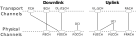
\includegraphics[width=0.95\columnwidth]{figures/chp_theory/complete.pdf}
    \caption{Mapping of transport channels to physical channels}
    \source{Created by the author based on \cite{ErikDahlman5G}}
    \label{fig:channel-mapping}
\end{figure}


Data in the transport channel is organized into transport blocks. For each component carrier and at each \gls{tti}, up to two \glspl{tb} are conveyed to the physical layer and transmitted over the radio interface  \cite{ErikDahlman5G}.
%
The transmission process is summarized in Figure \ref{fig:transmission}.
%
This process is similar for the uplink and downlink, the only difference being the additional step of transform precoding after the layer mapping in the uplink case.

\begin{figure}[htbp]
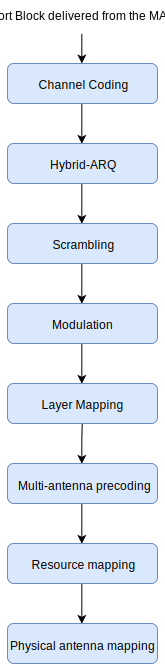
\includegraphics[width=\columnwidth]{figures/chp_theory/transmissionmodel.pdf}
\caption{General transmission model on \gls{5g} \gls{nr}}
\label{fig:transmission}
\end{figure}
%
In the modulation phase, \gls{nr} supports \gls{qpsk} and three orders of \gls{qam}, namely 16\gls{qam}, 64\gls{qam} and 256\gls{qam}, for both the uplink and downlink, with an additional option of $\pi/2$-BPSK in the uplink.
%
The \gls{fec} code for the \gls{embb} use case in data transmission is the \gls{ldpc} code, whereas in the control signaling polar codes are used.
%

In our work, we are mainly concerned with the \gls{pdsch} transmissions, in this case the overall \gls{5g} \gls{nr} channel coding process comprises six steps \cite{ErikDahlman5G}, namely:
\begin{itemize}
	\item \Gls{crc} Attachment: Calculates a \gls{crc} and attaches it to each transport block. It facilitates error detection and its size can be of 16 bits or 24 bits.
	\item Code-block segmentation: Segments the transport block in the case of it being larger in size than the supported by the \gls{ldpc} coder. Produces \gls{cb} are of equal size.
	\item Per-\gls{cb} \gls{crc} Attachment: A \gls{crc} is calculated and appended to each \gls{cb}.
	\item \gls{ldpc} Encoding: The solution used in \gls{nr} is a Quasi-cyclic \gls{ldpc} with two base graphs, the two base matrices that are used to built the different parity-check matrices with different payloads and rates.
	\item Rate Matching: It adjusts the coding to the allocated resources. It consists of bit selection and bit interleaving.
	\item Code-Block Concatenation: Concatenates the multiple rate-matching outputs into one block.
\end{itemize}

The other blocks in Figure \ref{fig:transmission}, excluding the channel coding and the modulation, are:
\begin{enumerate}
	\item \Gls{harq}: \gls{5g} \gls{nr} uses \gls{harq} with soft combining as the primary way to handle retransmissions. In this approach, a buffer is used to store the erroneous packet and this packet is combined with the retransmission to acquire a combined packet, which is more reliable than its components.
	%
	\item Scrambling: The process of scrambling is applied to the bits delivered by the \gls{harq}. Scrambling the bits makes them less prone to interference.
	%
	\item Layer mapping: The process of layer mapping is applied to the modulated symbols. It distributes the symbols across different transmission layers.
	%
	\item Multi-antenna precoding: This step uses a precoder matrix to map the transmission layers to a set of antenna ports.
	%
	\item Resource mapping: This process takes the symbols that should be transmitted by each antenna port and maps these to the set of available resource elements.
	%
	\item Physical antenna mapping: Maps each resource to a physical antenna.
\end{enumerate}

The \gls{pdsch} has only one defined transmission scheme \cite{3gpp.38.214}.
%
In this scheme the downlink transmission can be performed with up to 8 transmission layers on antenna ports 1000-1011.
%


In the following subsections we give an overview of the \gls{5g} \gls{nr} \gls{ldpc} coding solution and a more detailed explanation of some of the \gls{pdsch} procedures in Figure \ref{fig:transmission}.


%%%%%%%%%%%%%%%%%%%%%%%%%%%%%--subsection--%%%%%%%%%%%%%%%%%%%%%%%%%%%%%%%%%

\subsection{The \gls{5g} \gls{nr} \gls{ldpc}}

% %
% Before explaining the \gls{cb} segmentation and the \gls{ldpc} encoding, we will present some introduction to the coding solution applied to the \gls{embb} use case in the \gls{5g} \gls{nr}.
% %

\Gls{ldpc} codes are a class of linear block codes based on a sparse \gls{pcm}  originally proposed by Gallager \cite{gallager1962}.
%
Several standards have incorporated \gls{ldpc} codes, such as IEEE 802.11n, IEEE 802.16e (WiMAX) and \gls{dvb-s2} \cite{AliZaidi632018}.
%
In the third and forth generations (3G and 4G) turbo codes were the primary coding scheme \cite{Richardson2018} and were one of the candidates for the \gls{5g} \gls{nr} along with polar codes and \gls{ldpc} codes \cite{Hamidi8417496}.
%
The \gls{5g} \gls{nr} will make a transition on the error correcting codes with the \gls{ldpc} codes being used for the data channel and polar codes being used for the control information, on both the \gls{embb} and in the release-15 \gls{urllc} use cases \cite{bae_abotabl_lin_song_lee_2019}.

Although turbo codes and \gls{ldpc} codes have similar error-correcting capabilities \cite{ErikDahlman5G}, \gls{ldpc} codes provide the following advantages \cite{Hui2018}:

\begin{enumerate}
    \item Higher coding gains
    \item Lower error floors
    \item Higher achievable peak throughput
    \item Lower decoding complexity and improved decoding latency, particularly on high code rates
    \item Can achieve greater parallelism when decoding
\end{enumerate}

In a $(n, k)$ \gls{ldpc} code, the \gls{pcm} is a $ (n-k) \times n$ sparse matrix, with $k$ being the number of information bits and $n$ being the number of code-word bits, i.e information bits plus parity bits.
%
The sparseness of the \gls{pcm} enables a relatively simple decoding by making use of low-complexity iterative decoding algorithms.
%
The \gls{pcm} can also be represented by a graph connecting $n$ variable nodes with $(n-k)$ check nodes, the check nodes correspond to the parity-check equations.
%
In this graph there is an edge between a variable node and a check node if the corresponding entry on the \gls{pcm} is not-null \cite{Richardson2018}.
%
This bipartite graph representation is known as Tanner graph \cite{TannerGraph} and is the reason that the term \glsfirst{bg} is used in the \gls{nr} specifications.
%


The \gls{nr} \gls{ldpc} codes are \gls{qc} \gls{ldpc} codes, a class of photograph codes \cite{bae_abotabl_lin_song_lee_2019}.
%
In \gls{qc}-\gls{ldpc} the \gls{pcm} is constructed based on a smaller photograph, also called base matrix or \gls{bg}, that describes the macroscopic structure of the code \cite{Richardson2018}.
%
The \gls{pcm} can then be constructed by replacing each entry of the base matrix by a $\gls{not:lift-factor} \times \gls{not:lift-factor} $ cyclic permutation matrix, this process is called lifting and $\gls{not:lift-factor}$ is the lifting size.
%
In a Tanner graph representation, the lifting procedure is equivalent to having the larger graph being formed by $\gls{not:lift-factor}$ copies of the \gls{bg} and permuting the edges \cite{bae_abotabl_lin_song_lee_2019}.
%
One important consequence of this structure is that, with the higher possible parallelism, the decode complexity is a function of the \gls{bg} size, not of the actual \gls{pcm} size, since it can be achieved a degree of parallelism of $\gls{not:lift-factor}$ \cite{bae_abotabl_lin_song_lee_2019}.
% The \gls{nr} specifies the maximum $\gls{not:lift-factor}$ to $384$.

% TODO: Figure of tanner graph here


In the \gls{5g} \gls{nr} \gls{ldpc} code, each ``0'' in the \gls{bg} is replaced by a $\gls{not:lift-factor} \times \gls{not:lift-factor} $ all-zero matrix and each ``1'' is replaced by a circularly shifted identity matrix, shifted by the corresponding shifting coefficient \cite{ErikDahlman5G}.
%
In the technical specification \cite{3gpp.38.212}, 51 lifting sizes are specified and they are divided in 8 groups, called set index $\gls{not:set-index}$, each set index corresponds to a different permutation design, i.e different shifting coefficients, this structure is resumed in the Table \ref{tab:lift-table}.
%
This design means that there are 51 \glspl{pcm} for each of the two \glspl{bg}.

\begin{table}[htb]
\centering
\caption{Sets of \gls{ldpc} lifting sizes}
\label{tab:lift-table}
\begin{tabular}{l c}
  \toprule
  Set index $\gls{not:set-index}$   & Set of lifting sizes $\gls{not:lift-factor}$ \\
  \midrule
  0  &  2, 4, 8, 16, 32, 64, 128, 256 \\
  1  &  3, 6, 12, 24, 48, 96, 192, 384 \\
  2  &  5, 10, 20, 40, 80, 160, 320 \\
  3  &  7, 14, 28, 56, 112, 224 \\
  4  &  9, 18, 36, 72, 144, 288 \\
  5  &  11, 22, 44, 88, 176, 352 \\
  6  &  13, 26, 52, 104, 208 \\
  7  &  15, 30, 60, 120, 240 \\
  \bottomrule
\end{tabular}
\source{\cite[Table 5.3.2-1]{3gpp.38.212}}
\end{table}


Two \glspl{bg} are specified in \gls{5g} \gls{nr}, in order to guarantee efficiency for all the payload sizes and code rates.
%


%%%%%%%%%%%%%%%%%%%%%%%%%%%%%--subsection--%%%%%%%%%%%%%%%%%%%%%%%%%%%%%%%%%
\subsection{\Acl{mcs} and \acl{tbs} determination}

To start the decoding process the \gls{ue} must first determine the modulation order, the target code rate and the \glspl{tbs} in the \gls{pdsch}.
%
To determine this the \gls{ue} needs some information:

\begin{enumerate}
    \item The \gls{mcs} index, $I_{mcs}$, which is a 5-bit field in the \gls{dci}.
    %
    \item The redundancy version, which is used for the \gls{harq} functionality on the rate-matching step of the channel coding and is a 2-bit field included in the \gls{dci}.
    %
    \item The number of layers.
    \item The number of allocated \glspl{prb} before the rate matching.
\end{enumerate}

The \gls{mcs} index is used alongside a table to determine the modulation order and the target code rate.
%
Until the writing of this work only three \gls{mcs} tables were defined in the the technical specification \cite{3gpp.38.214}, two of modulation order up to 64\gls{qam}, with one of those used for a low spectral efficiency case, and one with modulation order going up to 256\gls{qam}.
%
In this work we used the table \cite[Table 5.1.3.1-2]{3gpp.38.214}, that goes up to 256\gls{qam}, reproduced in Table \ref{tab:mcs-table}, where \gls{not:rate} is the target code rate:

\begin{table}[htb]
\centering
\caption{\gls{mcs} index table 2 for \gls{pdsch}}
\label{tab:mcs-table}
\begin{tabularx}{0.95\columnwidth}{l X X r}
  \toprule
  \gls{mcs} index  & Modulation order & \gls{not:rate} x 1024  &  Spectral efficiency \\
  \midrule
  0  &  2   & 120       &  0.2344 \\
  1  &  2   & 193       &  0.3770 \\
  2  &  2   & 308       &  0.6016 \\
  3  &  2   & 449       &  0.8770 \\
  4  &  2   & 602       &  1.1758 \\
  5  &  4   & 378       &  1.4766 \\
  6  &  4   & 434       &  1.6953 \\
  7  &  4   & 490       &  1.9141 \\
  8  &  4   & 553       &  2.1602 \\
  9  &  4   & 616       &  2.4063 \\
  10 &  4   & 658       &  2.5703 \\
  11 &  6   & 466       &  2.7305 \\
  12 &  6   & 517       &  3.0293 \\
  13 &  6   & 567       &  3.3223 \\
  14 &  6   & 616       &  3.6094 \\
  15 &  6   & 666       &  3.9023 \\
  16 &  6   & 719       &  4.2129 \\
  17 &  6   & 772       &  4.5234 \\
  18 &  6   & 822       &  4.8164 \\
  19 &  6   & 873       &  5.1152 \\
  20 &  8   & 682.5     &  5.3320 \\
  21 &  8   & 711       &  5.5547 \\
  22 &  8   & 754       &  5.8906 \\
  23 &  8   & 797       &  6.2266 \\
  24 &  8   & 841       &  6.5703 \\
  25 &  8   & 885       &  6.9141 \\
  26 &  8   & 916.5     &  7.1602 \\
  27 &  8   & 948       &  7.4063 \\
  28 &  2   & Reserved  & Reserved \\
  29 &  4   & Reserved  & Reserved \\
  30 &  6   & Reserved  & Reserved \\
  31 &  8   & Reserved  & Reserved \\
  \bottomrule
\end{tabularx}
\source{\cite[Table 5.1.3.1-2]{3gpp.38.214}}
\end{table}

The \gls{tbs} determination process is defined in \cite[Section 5.1.3.2]{3gpp.38.214}, and it depends on the following parameters:

\begin{enumerate}
    \item $N_{sc}^{RB}$: The number of subcarriers in a \gls{rb}, 12.
    \item $N_{symb}^{sh}$: Number of symbols of the \gls{pdsch} allocation within the slot.
    \item $N_{DMRS}^{PRB}$: Number of \glspl{re} for \gls{dmrs} per \gls{prb} in the scheduled duration including the overhead of the \gls{dmrs} \gls{cdm} groups without data.
    \item $N_{oh}^{PRB}$: Overhead configured by a higher layer parameter. Set to 0 if not configured.
    \item $n_{PRB}$: Total number of allocated \glspl{prb} for the \gls{ue}.
\end{enumerate}

With the above information, the total number of \glspl{re} in the \gls{pdsch} allocation can be determined, which will be used to calculate the \gls{tbs} using also the number of transmission layers, \gls{not:nLayers}, the target code rate, \gls{not:rate}, and the modulation order, \gls{not:mod}.

At the transmitter side, \gls{bs}, a \gls{tb} of size \gls{tbs} is delivered from the \gls{mac} to the \gls{phy} where the process of Figure \ref{fig:transmission} happens.

%%%%%%%%%%%%%%%%%%%%%%%%%%%%%--subsection--%%%%%%%%%%%%%%%%%%%%%%%%%%%%%%%%%

\subsection{\gls{crc} attachment}

The \gls{crc} bits are calculated from a cyclic generator polynomial.
%
In the \gls{pdsch} procedure there are three polynomials that can be used \cite{3gpp.38.212}:

\begin{equation} \label{eq.:crc24a}
    \begin{split}
        g_{\mathrm{CRC24A}}(D) = & [ D^{24} + D^{23} + D^{18} + D^{17} +  D^{14} + D^{10} \\ & + D^{7} + D^{7} + D^{5} + D^{4} + D^{3} + D + 1 ]
    \end{split}
\end{equation}

\begin{equation}\label{eq.:crc24b}
    g_{\mathrm{CRC24B}}(D) = \left[ D^{24} + D^{23} + D^{6} + D^{5} + D + 1 \right]
\end{equation}

\begin{equation} \label{eq.:crc16}
    g_{\mathrm{CRC16}}(D) = \left[ D^{16} + D^{12} + D^{5} + 1 \right]
\end{equation}


The \gls{crc} makes possible for the receiver to detect errors in the decoded \gls{tb}.
%
For each \gls{tb} delivered from the \gls{mac} to the \gls{phy} a \gls{crc} is calculated and attached to it.
%
In case the \gls{tbs} is greater than 3824, the \gls{crc} has a length of 24 bits with the generator polynomial $g_{\mathrm{CRC24A}}$, Equation \eqref{eq.:crc24a}, being used.
%
Generator polynomial $g_{\mathrm{CRC16}}$, Equation \eqref{eq.:crc16}, is used otherwise, producing a 16-bit \gls{crc}.

When \gls{cb} segmentation occurs each \gls{cb} receives a \gls{crc} of 24 bits, which is calculated from the generator polynomial $g_{\mathrm{CRC24B}}$, Equation \eqref{eq.:crc24b}.
%
This process is ilustrated in Figure \ref{fig:cbcrc}.
%
If only one \gls{cb} is produced, no additional \gls{crc} is attached to it \cite{ErikDahlman5G}.

\begin{figure}[htb]
    \includegraphics[width=\columnwidth]{figures/chp_theory/crc.pdf}
    \caption{\gls{crc} attachements and \gls{cb} segmentation}
    \label{fig:cbcrc}
\end{figure}


%




%%%%%%%%%%%%%%%%%%%%%%%%--End Of Section--%%%%%%%%%%%%%%%%%%%%%%%%%%%%%%
\section{Reinforcement Learning }
\label{sec:rl-theory}
\Gls{rl} is a \gls{ml} technique that aims to find the best behavior in a given situation in order to maximize a notion of accumulated reward \cite{Bishop07}.
%
Figure \ref{fig:rlbasic} shows a simple block diagram of the \gls{rl} problem in which an agent, which is the learner and decision maker, interacts with an environment by taking actions.
%
By its turn, the environment responds to these actions and presents new situations, as states, to the agent \cite{sutton2018rl}.
%
The environment also responds by returning rewards, which the agent tries to maximize by choosing its actions.
%
Unlike supervised learning, where the system learns from examples of optimal outputs, the \gls{rl} agent learns from trial and error, i.e., from its experience, by interacting with the environment.

\begin{figure}[htbp]
\centerline{\includegraphics[width=90mm]{figures/chp_theory/rl-model.pdf}}
\caption{Basic diagram of a \gls{rl} scheme}
\label{fig:rlbasic}
\end{figure}
% another intro:
% Reinforcement Learning (RL) is a machine Learning tech-
% nique that aims to find the best behavior in a given situation
% in order to maximize a notion of accumulated reward [8].
% Figure 1 shows a simple block diagram of RL problem, in
% which an agent interacts with an environment by taking actions
% and evaluating the results of these actions, these results are
% perceived by the agent as a new state and by a received reward
% signal. Unlike supervised learning, where the system learns
% from examples of optimal outputs, the RL agent learns from
% trial and error.

At each time step $t$, the agent receives the state of environment $s_t \in \mathcal{S}$, and based on that chooses an action $a_t \in \mathcal{A}$.
%
As consequence of its action, the agent receives a reward $r_{t+1} \in \mathcal{R} $, with $\mathcal{R} \subset \mathbb{R}$, and perceives a new state $s_{t+1}$.
%
In light of this, the basics components of a \gls{rl} problem are:

\begin{itemize}
  \item State Space $\mathcal{S}$: Set of all possible states that can be observed by the agent. The random variable $S_t$ denotes the state at time step $t$ and a sample of $S_t$ is denoted $s_t$, with $s_t \in \mathcal{S}$.
  \item Action Space $\mathcal{A}$: Set of all actions that can be taken by agent. The random variable $A_t$ denotes the action at time step $t$ and a sample of $A_t$ is denoted $a_t$, with $a_t \in \mathcal{A}$
  \item Transition Probability Space $\mathcal{P}: \mathcal{S} \times \mathcal{A} \times \mathcal{S} \rightarrow [0;1]$ is the transition model of the system, $p(s_{t+1} | s_t,a_t) \in \mathcal{P}$ is the probability of transitioning to state $s_{t+1}$ after taking action $a_t$ in state $s_t$.
  \item Reward  $r_t$: This value indicates the immediate payoff from taking an action $a_t$ in a state $s_t$. $R_t$ is a random variable with a probability distribution depending only of the preceding state and action. We define the expected reward obtained from taking an action $a_t$ in a state $s_t$ as $r(s_t,a_t) = \mathbb{E}\left[R_{t+1} \, | \, S_t = s_t, A_t = a_t \right] $.
  \item Policy $\pi(s_t) \in \mathcal{A} $: The policy maps the states to actions. More specifically, it maps the perceived states of the environment to the actions to be taken by the agent in those states. The policy can also be defined as $\pi(a_t | s_t)$, the probability of selecting action $a_t$ given the agent is at a state $s_t$.
  % different policies can give different probabilities to each action.
  \item Q-function $Q^{\pi}(s_t,a_t)$:  The Q-Function, called action-value function, is the overall expected reward for taking an action $a_t$ in a state $s_t$ and then following a policy $\pi$. It can also be simply denoted as $Q(s_t,a_t)$.
\end{itemize}


The goal of the \gls{rl} agent is to find the optimal policy $\pi^{*}(s_t)$, whose state-action mapping leads to the maximum long term reward given by $G_t = \sum_{t=0}^{\infty} \gamma^{t} r_{t+1} = r_{t+1} + \gamma G_{t+1} $ \cite{kaelbling1996reinforcement}, where $r_t$ is the received reward at time step $t$.
%
The agent finds its best policy by taking into consideration the value of the Q-function to a state-action pair.
%
Mathematically, the Q-Function is defined as \cite{2010Szepesvari}:
\begin{equation} \label{eq.:eqQvalue}
  Q^{\pi}(s_t, a_t)=\mathbb{E}\left[\sum_{k=0}^{\infty} \gamma^{k} R_{t+k+1} \, | \, S_t = s_t, A_t = a_t \right], s_t \in \mathcal{S}, a_t = \pi (s_t) \in \mathcal{A}
\end{equation}


The parameter $\gamma$ is called \textit{discount factor}, or discount rate, with $0 \leq \gamma \leq 1$.
%
The discount factor is used to control the importance given to future rewards in comparison with immediate rewards, so a reward received $k$ time steps later is worth only $\gamma^{k-1}$ times its value.
%
The infinity sum $\sum_{t=0}^{\infty} \gamma^{t} r_{t+1}$ has a finite value if $\gamma \leq 1$, as long as the sequence $\{r_k\}$ is bounded \cite{sutton2018rl}.
%
The process is called undiscounted if $\gamma=1$.


The Q-values in successive steps are related according to the Bellman equation:
\begin{equation} \label{eq.:bellmanEq}
  %\begin{split}
    Q^{\pi}(s_t, a_t)= \sum_{s_{t+1} \in \mathcal{S}} p\left(s_{t+1} \, | \, s_t , a_t \right) \bigg[ r\left(s_t, a_t \right)  +
    \gamma \sum_{a_{t+1} \in \mathcal{A}} \pi\left(a_{t+1} \, | \, s_{t+1}\right) Q^{\pi}\left(s_{t+1}, a_{t+1}\right)  \bigg]
  %\end{split}
\end{equation}

The Equations \eqref{eq.:eqQvalue} and \ref{eq.:bellmanEq} can be rewritten for the case of $\pi$ being the optimal policy.
%
In this case, Equation \eqref{eq.:eqQvalue} leads to \cite{sutton2018rl}:

\begin{equation} \label{E_Optimal}
    Q^{\pi^*}\left(s_t, a_t\right)=\mathbb{E}\left[R_{t+1}+\gamma \max _{a_{t+1} \in \mathcal{A}} Q^{\pi^*}\left(S_{t+1}, a_{t+1}\right) \, | \, S_t=s_t, A_t=a_t\right]
\end{equation}

Likewise, assuming the optimal policy, Equation \eqref{eq.:bellmanEq} leads to \cite{DRL_AMC}:

\begin{equation} \label{eq.:bellmanOptimal}
    Q^{\pi^*}\left(s_t, a_t\right)=r(s_t,a_t)+ \gamma \sum_{s_{t+1} \in \mathcal{S}} p\left(s_{t+1} \, | \, s_t,a_t\right) \max _{a_{t+1} \in A} Q^{\pi^*}\left(s_{t+1}, a_{t+1}\right)
\end{equation}


Equation \eqref{eq.:bellmanOptimal} can only be solved if we know the transition probabilities.
%
However, if we don't have an adequate model of the environment the agent can take actions and observe their results, then it can fine-tune the policy that decides the best action for each state.
%
The algorithms that explore the environment to find the best policy are called model-free, while those ones that use the transition probabilities are called model-based.


\subsection{Exploration and Exploitation Trade-off}

One of the main paradigms in \gls{rl} is the balancing of exploration and exploitation.
%
The agent is exploiting if is choosing the action that has the greatest estimate of action-value, these are usually called the greedy actions.
%
Whereas exploring is when the agent chooses the non-greedy actions, to improve their estimates.
%
This leads to a better decision-making because of the information the agent has about these non-greedy actions \cite{sutton2018rl}.
%


There are different strategies to control the exploring and exploiting trade off. The reader have a deep discussion on that topic in \cite{exploration2016}.
%
In this work, we make use of two strategies:
\begin{enumerate}
  \item $\epsilon$-greedy: One of the most common exploration strategies. It selects the greedy action with probability $1-\epsilon$, and a random action with probability $\epsilon$. So, a higher $\epsilon$ means that the agent give more importance to exploration.
  \item adaptive $\epsilon$-greedy: There are numerous different methods that adapt the $\epsilon$ over time or as a function of the error \cite{improvingBandits}.A commonly used approach is to start with a high $\epsilon$ and decrease it over time.
%   \item Boltzmann exploration: Also known as softmax exploration. It uses the action-values to choose an action according to the Boltzmann distribution:
%   $$
% \pi\left(s, a\right)=\frac{e^{Q\left(s, a\right) / T}}{\sum_{i=1}^{m} e^{Q\left(s^{\prime}, a_i\right) / T}}
%   $$
%   The parameter $T \geq 0$, called temperature, sets the balance between exploration and exploitation. If $T \rightarrow 0$  the agent will only exploit, if $T \rightarrow \infty$ the agent will choose actions at random.
\end{enumerate}


\subsection{Q-Learning}

In this work, we adopt the Q-learning algorithm, which is an off-policy temporal difference (TD) algorithm.
%
TD methods are model-free and they update their estimates partially based on other estimates, without the need to wait for a final outcome \cite{sutton2018rl}.
%
An off-policy method can learn about the optimal policy at the same time it follows a different policy, called the behavior policy.
%
This behavior policy still has an effect on the algorithm, because it determines the choices of actions. The basic form of the action-values updates is:
\begin{equation}\label{QlearningEq}
%  \begin{split}
    Q\left(s_{t}, a_{t}\right) \leftarrow  (1-\alpha) Q\left(s_{t}, a_{t}\right)
    +\alpha\left[r_{t+1}+\gamma \max _{a_{t+1} \in A} Q\left(s_{t+1}, a_{t+1}\right)\right],
%  \end{split}
\end{equation}

\noindent where the parameter $0 \leq \alpha \leq 1$ is called learning rate.
%
% The Algorithm \ref{alg1} details Q-learning algorithm \cite{sutton2018rl}.
%
% \begin{algorithm}[htb]
%
% Algorithm parameters: step size $\alpha \in (0, 1]$, small $\epsilon > 0$\;
% Initialize $Q(s, a)$, for all $s \in \mathcal{S}, a \in \mathcal{A}$\;
% \ForEach{iteration}{
% Initialize s\;
%   Choose $a$ from $s$ using policy derived from $Q$ (e.g., $\epsilon$-greedy)\;
%   Take action $a$, observe $r$, $s^{\prime}$\;
%   $Q(s, a) \leftarrow (1-\alpha) Q(s, a) + \alpha [r + \gamma \max_a Q(s',a)]$\;
%   $s \leftarrow s^{\prime}$\;
%
% }
% \caption{Q-learning (off-policy TD control) for estimating $\pi \approx \pi^* $}
%   \label{alg1}
% \end{algorithm}


\chapter{\Acl{amc}}
\label{chp:amc}
% \section{Introduction}
% \label{sec:amc-intro}
%
%
% Link adaptation is a key enabling technology for broadband mobile internet, and has been part of the \gls{5g} \gls{nr} access technology.
% %
% In this context, \gls{amc} refers to the selection of the appropriate \gls{mcs} as a function of the channel quality, in order to keep the \gls{bler} below a predefined threshold.
% %
% In 4G long term evolution (LTE), the \gls{bler} target is fixed at 10\% \cite{3gpp.36.213}. However, 5G systems will cover a wider spectrum of services, requiring potentially different \gls{bler} targets \cite{Amin_2016,fantacci2009adaptive}.
%
% %
% % \Gls{5g} wireless communication systems are being designed to provide high data and transmission rates \cite{Amin_2016}.
% % %
% % Because of this, a reliable link adaptation process for \gls{5g} \gls{nr} is needed for coping with the need of increasing the data rate that can be accurately transmitted \cite{chu01}.
% % %
% %
% % In this context, the link adaptation technique of \gls{amc} is of great interest.
% % %
% % \Gls{amc} is a resource allocation technique used in link adaptation that allows the system to select the most appropriate \gls{mcs} to better cope with the changing channel conditions \cite{fantacci2009adaptive}.
% % %
%
% \Gls{amc} is a good solution to match the link throughput to the time-varying nature of the wireless channel under mobility.
% %
% Periodically, the \gls{ue} measures the channel quality and maps this information into a \gls{cqi}.
% %
% The \gls{bs} uses the \gls{cqi} reported by the \gls{ue} to define the \gls{mcs}.
% %
% Typically, each \gls{cqi} is associated with a given \gls{snr} interval \cite{Blanquez-Casado2016}.
% %
% Considering \gls{lte} as an example, the \gls{bs} uses \gls{dci} embedded into the \gls{pdcch} to inform the \gls{ue} about each new \gls{mcs} selection \cite{ErikDahlman5G}.
%
% %
% % In the downlink \gls{amc} procedure, the \gls{ue} suggests to the \gls{bs} an appropriate \gls{mcs} in the \gls{amc} set to be used \cite{Sang2014}.
% % %
% % This proposed \gls{mcs} is informed to the \gls{bs} by means of a \gls{cqi}, typically each \gls{cqi} represents a \gls{snr} interval \cite{Blanquez-Casado2016}.
% % %
% % In possession of this information, the \gls{bs} selects an \gls{mcs} to transmit and reports  its selection to the \gls{ue}.
%
% Conventional solutions to the \gls{amc} problem includes the fixed look-up table \cite{fantacci2009adaptive}, also called \gls{illa}, and the \gls{olla} technique, which further improves the look-up table by adapting the \gls{snr} thresholds.
% %
% The \gls{olla} technique was first proposed in \cite{Sampath1997}, and was also addressed in \cite{Pedersen2007,Sarret2015, Blanquez-Casado2016}.
%
% \Gls{ml} has become an attractive tool to devise novel \gls{amc} solutions in the context of complex emerging \gls{5g} systems and services.
% %
% In particular the drive towards self-organizing networks is potentially addressed by machine learning.
% %
% While in \gls{lte}, a look-up table provides fixed \gls{amc} rules for all the users, the emerging systems need a more flexible approach that can automatically adjust physical layer parameters (such as the modulation and coding scheme) according to the user channel state and service type.
% %
% \Gls{rl} refers to a category of \gls{ml} techniques \cite{survey-son} that has been applied to problems such as backhaul optimization~\cite{jaber2015}, coverage and capacity optimization~\cite{Fan2014} and resource optimization~\cite{Miozzo2017SwitchOnOffPF}.
% % The goal of the \gls{amc} is an automatic choice of the best parameters, in this case the \gls{mcs}, depending on the user and applications requirements.
% % %
% % As such, \gls{ml} algorithms are well suited to this application, because of their capabilities of learning patterns, forecasting behaviors and generating models \cite{survey-son}.
% %
% % A \gls{ml} category of particular interest to cellular systems is the \gls{rl}, because of its applicability in optimization problems \cite{survey-son}, such as backhaul optimization~\cite{jaber2015}, coverage and capacity optimization~\cite{Fan2014} and resource optimization~\cite{Miozzo2017SwitchOnOffPF}.
% There are few works that use \gls{rl} to solve the \gls{amc} problem.
% %
% In \cite{continuousState}, the selection of the \gls{mcs} is based on the received \gls{sinr}.
% %
% In this case, the state space is continuous, and the learning algorithm must handle a large state space.
% %
% In \cite{bruno2014robust} a Q-learning algorithm is proposed to solve the \gls{amc} problem in the context of a 4G \gls{lte} network.
% %
% A deep reinforcement learning approach is adopted in \cite{DRL_AMC} in the context of a cognitive heterogeneous network.
% %
%
%
% This work proposes a novel 5G \gls{amc} solution based on a \gls{rl} framework.
% %
% The proposed solution consists of collecting channel measurements at specific time instants to train an agent using the Q-learning algorithm.
% %
% The trained agent selects  a \gls{mcs} according to SNR measurements to maximize the current spectral efficiency.
% %
% We assume  a beam-based \gls{5g}-\gls{nr} as access technology, where the transmit and receive beams are selected using the beam sweeping procedure from \cite{giordani21}. The proposed \gls{amc} acts between any two consecutive points of sweeping.
% %
% We consider that the \gls{snr} between two consecutive points of sweeping tends to decrease due to the \ue~mobility  since it causes a mismatch among beams and the channel paths.
% %
% The agent uses the trained Q-table and the current measured \gls{snr} to properly select a \gls{mcs}.
% %
% To the best of authors' knowledge, previous works in \gls{amc} do not address the mismatch among beams and channel paths, while our solution works within the 5G-NR framework.
%%%%%%%%%%%%%%%%%%%%%%%%%%%%%%%%%%--End Of Section--%%%%%%%%%%%%%%%%%%%%%%%%%%%%%%%%%%%%%

\section{System Model}
\label{sec:amc-system-model}
%\subsection{Signal Model}

Consider a single cell system whose \gls{bs} is equipped with \gls{not:txAnt} antennas serving one \gls{ue} with \gls{not:rxAnt} antennas. The signaling period, of duration $T_{SS}$ herein referred to as a \emph{frame}, is divided into two time windows, as shown in Figure \ref{fig:amc-system-timing}. The first one contains a set of synchronization signal (SS) blocks with duration $T_{BS}$, where \emph{beam sweeping} is performed. More specifically, during this time window, the search for the best beam pair happens. The second time window is dedicated to data transmission using the selected beam pair. During this period, of duration $T_{D}$, the UE reports periodically the measured CQI to the BS that responds with the selected MCS.
%
%Assume that the user is synchronized with the  \gls{bs}, and they periodically measure their associated \gls{not:nBeams}  beam pairs.
%Assume that the \gls{bs} sends periodically synchronization signal (SS) blocks used by the \gls{ue} to measure a set of beam pairs and then selecting that one with highest \gls{snr}.
%
%The \base~and \ue~are assumed to apply \gls{not:Wtx} \inSetComplex{\gls{not:txAnt}}{\gls{not:nBeams}} and \gls{not:Wrx} \inSetComplex{\gls{not:rxAnt}}{\gls{not:nBeams}}, respectively.

During the transmission of the SS blocks, the BS measures all possible combinations of transmit and receive beams from the codebooks \gls{not:Wtx} \inSetComplex{\gls{not:txAnt}}{\gls{not:nBeams}} and \gls{not:Wrx} \inSetComplex{\gls{not:rxAnt}}{\gls{not:nBeams}}, respectively,  to select the beam pair with the highest \gls{snr}.
%
The selected beam pair for the $k$-th frame is expressed as
\begin{equation}
\label{eq.:amc-beam-sweeping}
  \{ \bar{\mathbf{w}}_k, \bar{\mathbf{f}}_k \}= \argmax_{\mathbf{w}, \mathbf{f}} \frac{\|\mathbf{w}^H \mathbf{H}_t \mathbf{f}\|}{\sigma ^2},
\end{equation}
%
\noindent where $\mathbf{f}$ and $\mathbf{w}$ are columns of \gls{not:Wtx} and \gls{not:Wrx}, respectively,  $\channel _t $ \inSetComplex{\gls{not:rxAnt}}{\gls{not:txAnt}} is the channel between the \base~ and the \ue at time $t$. We assume that the channel remains constant during the beam sweeping period $T_{BS}$.
%
The update of $\{ \bar{\mathbf{w}}_k, \bar{\mathbf{f}}_k \}$ depends on the periodicity $T_{SS}$ of the synchronization signal blocks, which can be  \{5, 10, 20 , 40, 80, 160\} (ms) \cite{giordani21}.
%
Therefore, the each beam pair solution remains constant within the time period $T_{SS}$, until the subsequent SS block arrives, when the BS can reevaluate Eq. \eqref{eq.:amc-beam-sweeping}.
%
%This process is illustrated in Figure \ref{fig:system-timing} that shows the measurement window model, where the \gls{mcs} decision points are the points in which the \gls{bs} and the \gls{ue} exchange information to choose the best \gls{mcs}, as explained in Section \ref{subsec:trans}.


%% explanation of figure
\begin{figure}[tb]
\centerline{\includegraphics[width=0.7\columnwidth]{figures/chp_amc/amc_q_learning.pdf}}
\caption{Model of time scheduling of operations.}
\label{fig:amc-system-timing}
\end{figure}


During the data transmission window, the discret-time received signal for the $t$-th symbol period associated with the $k$-th fixed beam pair, is given by
\begin{equation}
\label{eq.:amc-rx-signal}
	\gls{not:Y}_{k,t} =
    \bar{\mathbf{w}}^H_k \,
  \channel _t\,
   \bar{\mathbf{f}}_k \,
   \gls{not:sscl}_t
   % _\userIdx
 +
  \bar{\mathbf{w}}^H_k \;
  \gls{not:Z}_t,
\end{equation}

\noindent where $\gls{not:sscl}$ is the symbol transmitted to the \ue, and $\gls{not:Z}_t$ is the additive white Gaussian noise with zero mean and variance \gls{not:var}.
%
%Note that the index $k$ and index $t$ refer to distinct points in time, i.e. the transmit and receive beams can have a mismatch with channel paths depending on \ue~mobility.
%
Defining
\begin{equation}
  \tilde{h}_{k,t} =     \bar{\mathbf{w}}^H_k \,
  \channel _t\,
   \bar{\mathbf{f}}_k \, ,
\end{equation}
as the effective channel at time $t$, associated with the chosen beam pair $\{ \bar{\mathbf{w}}_k, \bar{\mathbf{f}}_k \}$, the effective SNR at the \ue \, is given by
%
\begin{equation}
    \label{eq.:amc-snr}
    \textrm{SNR} = \frac{ \abs{
    % \hermitian{\gls{not:Wrx}\subArg{\userIdx}\argPair{:}{\idxI}}
     \tilde{h}_{k,t}
      % \subArg{\userIdx} \gls{not:Wtx}\subArg{\userIdx}\argPair{:}{\idxJ}
      }^2 }{\gls{not:var}} p_{\gls{not:sscl}},
\end{equation}
%https://www.overleaf.com/project/5d16668cdc29bf0ff4f11132
where $p_{\gls{not:sscl}}$ is the the power of transmitted symbol.
%
%
%\noindent with \gls{not:Wrx}\subArg{\userIdx}\argPair{:}{\idxI} and \gls{not:Wtx}\subArg{\userIdx}\argPair{:}{\idxJ} being the \idxI th and \idxJ th beams of the codebook  \gls{not:Wrx}\subArg{\userIdx} and \gls{not:Wtx}\subArg{\userIdx}, respectively.

% \subsection{Channel Description}
%The model in \eqref{eq.:rx_signal} assumes a narrowband block-fading channel, so the channel is almost constant within a time-frequency resource block \cite{alkhateeb2014}.

\subsection{Channel Model}

We assume a geometric channel model with limited number \gls{not:scatterers} of scatterers.
%
Each scatterer contributes with a single path between \gls{bs} and \gls{ue}. Therefore, the channel model can be expressed as
%
\begin{equation}\label{eq.:amc-channelModel}
\channel _t= \sqrt{\pathloss}\sum_{i=0}^{\gls{not:scatterers} - 1 } \gls{not:beta}_i \strRx \anglePair{i,t}{ue} \hermitian{\strTx  \anglePair{i,t}{bs}} e^{ \mathrm{j} 2 \pi f_i tT_s} ,
\end{equation}
\noindent where $T_s$ is the \gls{ofdm} symbol period, $\pathloss$ denotes the pathloss, \gls{not:beta} is the complex gain of the $k$th path and $f_i$ is the Doppler frequency for the $i$th path.
%
The parameters \azm~$\in$ \range{0}{2\pi} and \elev~$\in$ \range{0}{\pi} denote the azimuth and elevation angles at the \base \, (\gls{aod}) and the \ue \, (\gls{aoa}).
%
We assume a \gls{ura}, the response of which is written as:
%
\begin{equation*}
  \begin{split}
    \strTx \anglePair{i,t}{bs} = & \frac{1}{\sqrt{\gls{not:txAnt}}} \bigg[ 1, \expUraPhase{}{i,t}{bs}, \\ & \ldots ,\expUraPhase{(\gls{not:txAnt} -1 )}{i,t}{bs} \bigg],
  \end{split}
\end{equation*}
where \dist ~is the antenna element spacing, and \wave~is the signal wavelength. The array response at \gls{ue} can be written similarly.

The expression in \eqref{eq.:amc-channelModel} can be expressed compactly as
\begin{equation}
\label{eq.:amc-channelModelMtx}
\channel _t = \strRxMtx \diag{\gls{not:betaVec}_t} \hermitian{\strTxMtx},
\end{equation}
where $\gls{not:betaVec}_t = \left[ \gls{not:beta}_0 e^{ \mathrm{j} 2 \pi f_0 t T_s}, \ldots, \gls{not:beta}_{\gls{not:scatterers}-1} e^{ \mathrm{j} 2 \pi f_{S-1} t T_s} \right]$, and the matrices \strRxMtx~and \strTxMtx~are formed by the concatenation of array response vector at the \base~and \ue, respectively.

\subsection{Transmission Model}
\label{subsec:la-trans}
The transmission process takes into account the channel coding and modulation blocks.
%
In this work, we implement all the steps specified in the \gls{nr} channel coding block except the rate matching \cite{3gpp.38.212}.
%
The \gls{cb} segmentation divides the transport block of $n_{bits}$ bits to fit the input size accepted by the \gls{ldpc} encoder, padding whenever necessary.
%
At the \gls{mcs} decision points, shown in Figure \ref{fig:amc-system-timing}, the  \gls{ue} reports the measured \gls{cqi} to the \gls{bs}, which decides the \gls{mcs} accordingly.
%
The selected \gls{mcs} is informed to the \gls{ue} through the \gls{pdcch} as a part of the \gls{dci}. This process is shown in Figure \ref{fig:amc-system-model}.
%

We considered a subset of the \gls{mcs}s in Table 5.1.3.1-1 in \cite{3gpp.38.214}, from the \gls{mcs} indexes 3 to 27. For our \gls{rl} based solution, the \gls{cqi} is a quantized measure of the \gls{snr}, and the number of possible \gls{cqi}s is defined by $N_{\text{cqis}}$. The \gls{cqi} metric for the \gls{rl}-\gls{amc} is defined as:
\begin{equation}\label{eq:amc-cqi}
    \textrm{CQI} =
    \begin{cases}
    0, \text{if } \textrm{SNR} \leq \textrm{SNR}_{\text{min}}\\
    (N_{\text{cqi}}-1), \text{if } \textrm{SNR} \geq \textrm{SNR}_{\text{max}}\\
    \floor[\Big]{\frac{(\textrm{SNR} - \textrm{SNR}_{\text{min}})(N_{\text{cqi}}-1)}{\textrm{SNR}_{\text{max}}-\textrm{SNR}_{\text{min}}}}
    \end{cases}
\end{equation}
\noindent Note that each \gls{cqi}, except the minimum and the maximum ones, comprises \gls{snr} intervals having the same length.
% , since the \gls{snr} inside the range $[snr_{min},snr_{max}]$ is divided equally into \gls{cqi}s in this calculation.

At each \gls{tti} the \gls{bs} makes a transmission of a \gls{tb} of $n_{bits}$ at the chosen \gls{mcs}. The \gls{ue} receives a \gls{tb} from the \gls{bs} and, in possession of the chosen \gls{mcs}, decodes the \gls{tb} and calculates its \gls{ber}, \gls{bler} and spectral efficiency.
%
%The \gls{ber} is the Hamming distance between the decoded \gls{tb} and transmitted \gls{tb}.
%
% The \gls{bler} is a ratio of blocks with \gls{ber} above $0.1$. The spectral efficiency $\eta$, in $bit/s/Hz$, is calculated in terms of number of bits per modulation symbol \gls{not:mod} and the code rate \gls{not:rate} as:
The \gls{bler} is the ratio of incorrectly received blocks over the total number of received blocks. %where a block is the result of the code block segmentation.
%
The spectral efficiency $\eta$, in $bit/s/Hz$, is calculated as:
\begin{equation}
 \label{eq.:spec-eff}
 \eta = (1-\textrm{\gls{bler}})\gls{not:mod}\gls{not:rate} \, ,
\end{equation}
\noindent where \gls{not:mod} is the number of bits per modulation symbol and \gls{not:rate} is the code rate.

\begin{figure}[htb]
\centerline{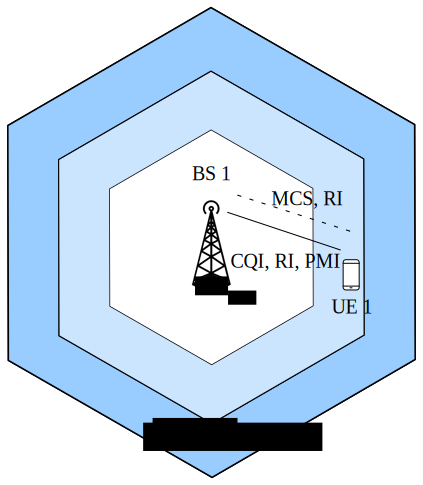
\includegraphics[width=0.4\columnwidth]{figures/chp_amc/system-model-mateus.pdf}}
\caption{Exchange of signals involved in the AMC procedure}
\label{fig:amc-system-model}
\end{figure}





%%%%%%%%%%%%%%%%%%%%%%%%%%%%%%%%%%--End Of Section--%%%%%%%%%%%%%%%%%%%%%%%%%%%%%%%%%%%%%

\section{Proposed Solution}

The proposed solution is a Q-learning based link adaptation scheme, herein referred to as \gls{ql-amc}.
%
In the proposed approach, the \gls{bs} selects the \gls{mcs} based on the state-action mapping obtained from the Q-learning algorithm.
%
More specifically, the \gls{bs} chooses the \gls{mcs} using the Q-table obtained from the \gls{rl} algorithm.
%
The \gls{rl} based solution enables the system to learn the particularities of the environment and adapt to it.

A diagram adapting the model from Figure \ref{fig:rlbasic} to the \gls{amc} problem is shown in Figure \ref{fig:amc-rl-frame}.
%
\begin{figure}[htb]
\centerline{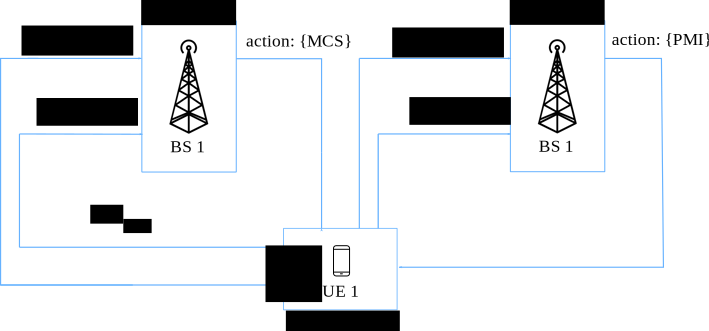
\includegraphics[width=0.5\columnwidth]{figures/chp_amc/rl-framework-mateus.pdf}}
\caption{Basic diagram of the proposed AMC scheme}
\label{fig:amc-rl-frame}
\end{figure}
%

In the proposed \gls{amc} problem, the state space is the set of all possible \gls{cqi}s, from $0$ to $(N_{\text{cqi}}-1)$; the action space is the set of all possible \gls{mcs}s. As for the reward, we consider two different metrics.
%
The first reward function is a non-linear one defined as:
\begin{equation}\label{eq.:rewardBler}
  R_1 = \begin{cases}
  \gls{not:mod} \gls{not:rate}, \text{ if } \textrm{BLER} \leq \textrm{BLER}_{\text{T}} \\
  -1, \text{ else.}
\end{cases}
\end{equation}
\noindent where \gls{not:mod} is the number of bits per modulation symbol, \gls{not:rate} is the code rate and $\textrm{BLER}_{\text{T}}$ is the target \gls{bler} of the system, $10\%$ in case of \gls{embb} \cite{3gpp.38.214}.
%
The goal of this reward function is to allow the agent to choose the best \gls{mcs} that satisfies the \gls{bler} target. The second reward is defined in terms of the spectral efficiency (in bits/second/hertz):
\begin{equation}\label{eq.:rewardSE}
    R_2 = (1-\textrm{BLER}) \gls{not:mod} \gls{not:rate} \text{.}
\end{equation}
\noindent With this function, the agent will try to maximize the spectral efficiency.
A summary of the proposed \gls{ql-amc} algorithm is shown in Algorithm \ref{amc-alg}.

\begin{algorithm}[htb]
  \caption{\strut QL-AMC}
    \label{amc-alg}
 \nonl Initialize $Q(s, a) = 0$, for all $s \in \mathcal{S}, a \in \mathcal{A}$\;
 \nonl \ForEach{MCS Decision Point (see Fig. \ref{fig:amc-system-timing})}{
  The UE \emph{observes the state} $s: $\gls{cqi} and feeds it back to the BS;\\
  The BS \emph{takes an action} $a: \textrm{MCS}$ using the policy driven by $Q$ (e.g., $\epsilon$-greedy);\\
  The BS \emph{perceives a reward} $r$ (c.f. Eqs. (\ref{eq.:rewardBler}) or (\ref{eq.:rewardSE})) and observes the next state $s^{\prime}$\;
  The BS update the Q-table: $Q(s, a) \leftarrow (1-\alpha) Q(s, a) + \alpha [r + \gamma \max_a Q(s',a)]$\;
  $s \leftarrow s^{\prime}$\;
\nonl }

\end{algorithm}


As will be shown in the next section, we will evaluate the impact and importance of on the system's \gls{bler} and spectral efficiency, and the difference between linear and non-linear rewards.

The Table \ref{tab:ql-amc-def} summarizes the definitions of state, action and reward.

\begin{table}[htb]
\centering
\caption{\gls{rl} elements}
\label{tab:ql-amc-def}
\begin{tabularx}{0.55\columnwidth}{X r}
\toprule
\textbf{Element} 	      & \textbf{Definition} \\
\midrule
State                   & \gls{cqi} \\
Action                  & \gls{mcs} \\
Reward                  & Eq: \eqref{eq.:rewardBler}, \eqref{eq.:rewardSE} \\
\bottomrule
\end{tabularx}
\end{table}
%

%%%%%%%%%%%%%%%%%%%%%%%%%%%%%%%%%%--End Of Section--%%%%%%%%%%%%%%%%%%%%%%%%%%%%%%%%%%%%%

\section{Simulations and Results}
\label{sec:amc-simulation}
\subsection{Simulation Parameters}
We assess the system performance with one \gls{bs} that serves one \gls{ue}.
%
The system has a bandwidth $B$ with a frequency carrier of $28$ GHz. Each resource block has a total of $12$ subcarriers and a subcarrier spacing $\gls{not:sub-spacing}= 120 \text{KHz}$.
%
%The frame is composed by 10 subframes, and each subframe is composed of multiple slots, where each slot has 14 symbols.
We consider the channel model defined in \eqref{eq.:amc-channelModel}.
%
The path loss follows a urban macro (UMa) model with non-line-of-sight (NLOS). Shadowing is modeled according to a log-normal distribution with standard deviation of $6$ dB \cite{AliZaidi632018}.
%
The noise power is fixed at $-123.185$ dBm.
%
A summary of the main simulation parameters is provided in Table~\ref{tab:amc-sim-params}, while the parameters of the proposed \gls{ql-amc} algortihm are listed in Table \ref{tab:amc-rl-params}.


\begin{table}[htb]
\centering
\caption{Simulation Parameters}
\label{tab:amc-sim-params}
\begin{tabularx}{0.8\columnwidth}{X r}
\toprule
\textbf{Parameter} 	& \textbf{Value} \\
\midrule
\gls{bs} height & 15 m\\
\gls{ue} height & 1.5 m\\
\gls{ue} track & rectilinear\\
\gls{bs}  antenna model & omnidirectional \\
\gls{bs}  antennas & 64 \\
\gls{ue} antenna model & omnidirectional \\
\gls{ue} antennas & 1 \\
Transmit power & 43 dBm\\
Frequency & 28 GHz\\
Bandwidth & 1440 MHz\\
Number of subcarriers  & 12\\
Subcarrier spacing & 120 kHz\\
Number of subframes & 10\\
Number of symbols & 14\\
Number of information bits per TTI & 1024\\
Azimuth angle spread & $[-60^{\circ}, 60^{\circ}]$\\
Azimuth angle mean & $0^{\circ}$\\
Elevation angle spread & $[60^{\circ}, 120^{\circ}]$\\
Elevation angle mean & $90^{\circ}$\\

Number of paths & 10\\
Path loss & UMa NLOS\\
Shadowing standard deviation & 6 dB\\
%Noise spectral density & -123 & dBm/Hz\\
\bottomrule
\end{tabularx}
\end{table}
%


\begin{table}[htb]
	\centering
	\caption{QL-AMC Parameters}
	\label{tab:amc-rl-params}
	\begin{tabularx}{0.8\columnwidth}{l r}
		\toprule
		\textbf{Parameter} 	   & \textbf{Value} \\
    \midrule
    $\textrm{SNR}_{\text{min}}$ for Eq. \eqref{eq:amc-cqi} & $-5$ \\
    $\textrm{SNR}_{\text{max}}$ for Eq. \eqref{eq:amc-cqi} & $40$ \\
		Discount factor ($\gamma$) & 0.10\\
		Learning rate ($\alpha$) & 0.90\\
		Maximum exploration rate ($\epsilon_{\max}$) & 0.50\\
    Minimum exploration rate ($\epsilon_{\min}$) & 0.05\\
    Cardinality of state space & $\{10,15,30,60 \}$\\
		\bottomrule
	\end{tabularx}
\end{table}

\subsection{Baseline Solutions}

% We compare the \gls{ql-amc} against the \gls{amc} based on the channel state \cite{fantacci2009adaptive} and target \gls{bler}, which produces a look-up table and also against the \gls{olla} technique \cite{Sarret2015}.
%
We compare the \gls{ql-amc} against the \gls{amc} based on a fixed look-up table \cite{fantacci2009adaptive} and also against the \gls{olla} technique from \cite{Pedersen2007}.
% We consider two fixed \gls{mcs}, the first is the QPSK with code rate of $1/3$ and the second is 16\gls{qam} with rate of $2/3$. In the results they are referred as "fixed 1" and "fixed 2".
%
In the fixed look-up table approach, a static mapping of \gls{snr} to \gls{cqi} is obtained by analyzing the \gls{bler} curves and selecting the best \gls{mcs}, in terms of throughput, that satisfies the target \gls{bler} \cite{bruno2014robust}.
%
The process of analyzing the \gls{bler} curves gives the \gls{snr} thresholds that separate each \gls{cqi}, as such the \gls{snr} to \gls{cqi} mapping for the look-up table and the \gls{olla} algorithm is different from the \gls{ql-amc} defined in Eq. \eqref{eq:amc-cqi}.
%
We assumed a direct mapping of \gls{cqi} to \gls{mcs}, i.e., each \gls{cqi} is mapped to one \gls{mcs} only .
% \begin{table}[tb]
% \centering
% \caption{Look-up Table}
% \label{tab:look-up}
% \begin{tabularx}{0.5\columnwidth}{l X r}
% \toprule
%  CQI   & Modulation   & Rate \\
% \midrule
%  0     & QPSK         & 1/3   \\
%  1     & QPSK         & 1/2   \\
%  2     & QPSK         & 2/3   \\
%  3     & 16QAM        & 1/2   \\
%  4     & 16QAM        & 2/3   \\
%  5     & 16QAM        & 3/4   \\
%  6     & 64QAM        & 2/3   \\
%  7     & 64QAM        & 3/4   \\
%  8     & 64QAM        & 5/6   \\
% \bottomrule
% \end{tabularx}
% \end{table}
The \gls{olla} technique consists of improving the conventional MCS look-up table by adjusting the \gls{snr} thresholds according to the \gls{acknack} from previous transmissions.
%
This adjustment is made by adding an offset to the estimated \gls{snr} to correct the \gls{mcs}s.
%
The \gls{snr} that is transformed to \gls{cqi} is:
\begin{equation}
\textrm{SNR}_{\text{olla}} = \textrm{SNR} + \Delta_{\text{olla}}
\end{equation}
\noindent where the $\Delta_{olla}$ is updated at each time step according to the Eq. \eqref{eq.:olla} \cite{Blanquez-Casado2016}:
\begin{equation}\label{eq.:olla}
  \Delta_{\text{olla}} \leftarrow \Delta_{\text{olla}} + \Delta_{\text{up}} \cdot e_{\text{blk}} - \Delta_{\text{down}} \cdot (1 - e_{\text{blk}}),
\end{equation}
\noindent where $e_{\text{blk}} = 1$ in case of NACK, or $e_{\text{blk}} = 0$ if the transmission is successful.
%
The parameters $\Delta_{\text{up}}$, $\Delta_{\text{down}}$ and the target \gls{bler}, $\textrm{BLER}_{\text{T}}$, are inter-related. In fact, by fixing the $\Delta_{\text{up}}$ and the $\textrm{BLER}_{\text{T}}$, the $\Delta_{\text{down}}$ can be calculated as \cite{Pedersen2007}:
$$
\Delta_{\text{down}} = \frac{\Delta_{\text{up}}}{\frac{1}{\textrm{BLER}_{\text{T}}} -1}.
$$
The target \gls{bler} for the \gls{olla} algorithm is fixed at $0.1$, while we assume three values for $\Delta_{\text{up}}$: 0.01dB, 0.1dB and  1dB.

\subsection{Experiment Description and Results}

The experiment devised to assess the performance of the \gls{ql-amc} in comparison to the baseline solutions (look-up table and OLLA) is composed of two phases, namely the learning phase and the deployment phase.
%
We also evaluate the effect of the type of reward function considered (i.e., Eqs. \eqref{eq.:rewardBler} or \eqref{eq.:rewardSE}), and the different number of \gls{cqi}s. As such, each \gls{ql-amc} configuration is defined in terms of the cardinality of the state space and the reward function.
%
The action space is the set of all possible modulations orders and code rates, being the same for all configurations.


\subsubsection{Learning Phase}
In the first phase, the \gls{rl} agent populates the Q-table to learn the environment.
%
Each configuration of the \gls{ql-amc} passes through this phase only one time. Our simulation time starts with the \gls{ue} positioned at a radial distance of $20m$ from the \gls{bs}. The UE moves away from the \gls{bs} up to a distance of 100m. Then, the \gls{ue} comes back to its original position following the same path in the reverse direction.
%
The \gls{ue} has a speed of $5km/h$ and the simulation runs for a time equivalent to $160s$ of the network time, which corresponds to the transmission of 32.000 frames.
%


%
The Table \ref{tab:amc-train-results} summarizes the results, providing average values, of the metrics for each configuration of the \gls{ql-amc}.
%
SE is the spectral efficiency given by Equation \eqref{eq.:spec-eff}.
%
\begin{table}[htb]
\centering
\caption{Training Phase Results}
\label{tab:amc-train-results}
\begin{tabularx}{0.75\columnwidth}{l X X X r}
\toprule
Length & Reward &  BLER &  SE &   BER \\
\midrule
10 &           2 & 0.0270 &  5.0850 & 0.0065 \\
10 &           3 & 0.0288 &  5.1696 & 0.0070 \\
15 &           2 & 0.0263 &  5.0827 & 0.0065 \\
15 &           3 & 0.0289 &  5.1054 & 0.0071 \\
30 &           2 & 0.0264 &  5.1463 & 0.0065 \\
30 &           3 & 0.0286 &  5.1227 & 0.0070 \\
60 &           2 & 0.0283 &  5.0852 & 0.0068 \\
60 &           3 & 0.0279 &  5.1701 & 0.0068 \\
\bottomrule
\end{tabularx}
\end{table}

Table \ref{tab:amc-train-results} reveals that configurations adopting the spectral efficiency (reward 2) as the reward function, with state space of lengths 10 or 60, achieve the best results in terms of spectral efficiency.
%
This is coherent since reward 2 is the own spectral efficiency.
%
When the performance metric is the \gls{bler}, the non-linear reward function (reward 1, Eq. \eqref{eq.:rewardBler}) provides the best results with lengths of 15 and 30.
%
Figures \ref{fig:amc-train-spceff} and \ref{fig:amc-train-bler} shows respectively the average spectral efficiency and the average \gls{bler} of these four possible configurations.
%
Figure \ref{fig:amc-train-spceff} shows that the length of the state space indeed has an important influence on the learning speed.
%
The smaller the length is, the faster is the learning speed, as expected.
%
The \gls{ql-amc} with length 60 has the worst performance before $10s$, but after $20s$ the performance of all configurations is approximately the same.
%

\begin{figure}[!htbp]
\centerline{\includegraphics[width=0.7\columnwidth]{figures/chp_amc/Spec-Eff-Train.pdf}}
\caption{Mean spectral efficiency on training phase}
\label{fig:amc-train-spceff}
\end{figure}

\begin{figure}[!htbp]
\centerline{\includegraphics[width=0.7\columnwidth]{figures/chp_amc/BLER-Train.pdf}}
\caption{Mean \gls{bler} on training phase}
\label{fig:amc-train-bler}
\end{figure}

The performances of the \gls{ql-amc}s in terms of \gls{bler} are similar for all configurations in Figure \ref{fig:amc-train-bler}.
%
Before the $20s$ mark the curves are close, whereas the configuration with length 10 degrades slightly compared to other configurations after this time mark.


\subsubsection{Deployment phase}
The second phase uses the knowledge from the first phase, but with an $\epsilon$-greedy policy with a fixed value of $\epsilon = 0.05$, accordingly to the minimum value of the $\epsilon$-decreasing in the training phase.
%
The goal is to have an assessment of how the \gls{rl} agent performs in the long run.
%

In the deployment phase, we compare the proposed \gls{ql-amc} solution with the baseline solutions (look-up table and OLLA).
%
We perform $200$ Monte Carlo runs. At each run, the \gls{ue} starts at a random position between $25m$ and $90m$ of the \gls{bs}.
%
The \gls{ue} moves in a random rectilinear direction with a random speed between $10km/h$ and $20km/h$. This corresponds to a total of $K=125$ frames. Recall that each frame comprises a beam sweeping procedure, followed by data transmission jointly with a MCS selection procedure, as shown in Figure \ref{fig:amc-system-timing}.
%


Table \ref{tab:amc-deploy-results} summarizes the results in the deployment phase in terms of average values for each configuration of the \gls{ql-amc} and baseline solution.
%
The first column represents the type of solution adopted.
%
% The two fixed \gls{mcs} schemes (denoted as "Fixed 1" and "Fixed 2") consider QPSK with code rate of 1/3 and 16QAM with code rate of 2/3, respectively.
%
We consider three \gls{olla} schemes, denoted as \gls{olla} 1, 2 and 3, which consider $\Delta_{\text{up}}$ 0.01dB, 0.1dB and 1dB, respectively.
%
The conventional \gls{amc} with a fixed look-up table is denoted as "Table".
%
The second column represents the number of \gls{cqi}s and the type column represents the reward function used, defined by Eqs. \eqref{eq.:rewardBler}, \eqref{eq.:rewardSE}, and denoted as \gls{bler} and SE.
%

\begin{table}[tb]
\centering
\caption{Deployment Phase Results (Average over 200 runs)}
\label{tab:amc-deploy-results}
\begin{tabularx}{\columnwidth}{l X X X X r}
  \toprule
  Type    & Cardinality &      Reward  &  BLER &     SE  &    BER \\
  \midrule
   QL-AMC &     10 &           BLER   & 0.0320 &  3.6700 & 0.0088 \\
   QL-AMC &     15 &           BLER   & 0.0306 &  3.3238 & 0.0087 \\
   QL-AMC &     30 &           BLER   & 0.0302 &  3.5594 & 0.0087 \\
   QL-AMC &     60 &           BLER   & 0.0306 &  3.8783 & 0.0087 \\
   QL-AMC &     10 &           SE     & 0.0306 &  3.9187 & 0.0086 \\
   QL-AMC &     15 &           SE     & 0.0301 &  3.8207 & 0.0085 \\
   QL-AMC &     30 &           SE     & 0.0310 &  3.9922 & 0.0086 \\
   QL-AMC &     60 &           SE     & 0.0311 &  4.1553 & 0.0086 \\
    Table &      - &           -      & 0.0311 &  3.8704 & 0.0088 \\
   OLLA 1 &      - &           -      & 0.0309 &  3.6700 & 0.0088 \\
   OLLA 2 &      - &           -      & 0.0330 &  1.8511 & 0.0090 \\
   OLLA 3 &      - &           -      & 0.0343 &  0.9999 & 0.0092 \\
  \bottomrule
\end{tabularx}
\end{table}

Analyzing Table \ref{tab:amc-deploy-results}, we see that the two \gls{ql-amc} configurations presenting the best results in terms of spectral efficiency are those with cardinality 30 and 60, adopting the reward function $R_1$ of Eq. \eqref{eq.:rewardSE}.
% %
% The knowledge learned in the training phase is passed through to the deployment phase, as these two configurations already demonstrated the best performance in the training phase.
%

\begin{figure}[tb]
\centerline{\includegraphics[width=0.7\columnwidth]{figures/chp_amc/SpecEff-Deploy.pdf}}
\vspace{-2ex}
\caption{CDF of average spectral efficiency (bps/Hertz)}
\label{fig:amc-dep-spceff}
\end{figure}

Figure \ref{fig:amc-dep-spceff} shows the cumulative distribution of the average spectral efficiency, in each Monte Carlo run, for the different \gls{ql-amc} configurations, with cardinality 30 and 60, which are labeled \gls{ql-amc} 1 and 2, respectively. We consider the reward function $R_2$ defined in Eq. \eqref{eq.:rewardSE}.
It can be seen that the proposed \gls{ql-amc} algorithm outperforms the baseline solutions in terms of spectral efficiency.
%comparison against to the baseline solutions.



%%%%%%%%%%%%%%%%%%%%%%%%%%%%%%%%%%--End Of Section--%%%%%%%%%%%%%%%%%%%%%%%%%%%%%%%%%%%%%


\section{Conclusions and Perspectives}
\label{sec:amc-conclusion}
We demonstrate through simulations that the \gls{rl} provides a self-exploratory framework that enables the \base~ to choose a suitable \gls{mcs} that maximizes the spectral efficiency.
%
Basically, the \gls{bs} decides a specific \gls{mcs} at a certain time instant. The \ue~ measures the reward of that action and report it to the \base.
%
Comparing with the fixed look-up table and \gls{olla} solutions, the proposed QL-AMC solution has achieved higher spectral efficiencies and lower BLERs.
%
Between the two rewards considered, the second one that is in function of the spectral efficiency has achieved the best performance.
%
As a perspective, we highlight extensions to multi-layer MIMO transmission. Moreover, a comparison with other RL-based algorithms such as multi-armed bandits (MABs) \cite{zhou2015survey} or deep RL solutions \cite{DeepRLSurvey} is envisioned.
%
% When considering multi-layer transmission, our \gls{rl}-based solution should be adapted to select both the \gls{amc} scheme and the number of spatial layers.
% %
% It is also worth mentioning that different spatial layers are associated with different \gls{cqi}s, which increases the number of possible actions and states of the proposed \gls{rl}-based \gls{amc} solution.
% %
% Hence, deep reinforcement learning should be investigated to deal with this increase in complexity.
%
% In addition, since \gls{nr} is a beam-based system, including the beam domain is another perspective.
% %
% In other words, our \gls{rl}-based solutions can also incorporate the selection of the best beam to transmit/receive data, among a set of choices (codebook).
% %
% These perspectives will be addressed in a follow-up work.

%%%%%%%%%%%%%%%%%%%%%%%%%%%%%%%%%%%%%%%%%%%%%%%%%%%%%%%%%%%%%%%%%%%%%%%%%%%%%%%%


\chapter{\Acl{la}} \label{chp:la}

Link adaptation


\chapter{Conclusions}% and Future Perspectives}
\label{chp:conclusion}
Final


% ----------------------------------------------------------
% ELEMENTOS PÓS-TEXTUAIS
% ----------------------------------------------------------
%\postextual

% Referências bibliográficas

\printbibliography

% Apêndices
% \appendix
% \include{chapters/appendix_RRMcomplexity}
%\end{otherlanguage*}


\end{document}
